% This is a LaTeX thesis template for Monash University.
% to be used with Rmarkdown
% This template was produced by Rob Hyndman
% Version: 6 September 2016

\documentclass{monashthesis}

%%%%%%%%%%%%%%%%%%%%%%%%%%%%%%%%%%%%%%%%%%%%%%%%%%%%%%%%%%%%%%%
% Add any LaTeX packages and other preamble here if required
%%%%%%%%%%%%%%%%%%%%%%%%%%%%%%%%%%%%%%%%%%%%%%%%%%%%%%%%%%%%%%%

\author{Huize Zhang}
\title{Exploration of Judicial Facial Expression in Videos of Legal Proceedings}
\studentid{27478343}
\def\degreetitle{Bachelor of Commerce (Honours)}
% Add subject and keywords below
\hypersetup{
     %pdfsubject={The Subject},
     %pdfkeywords={Some Keywords},
     pdfauthor={Huize Zhang},
     pdftitle={Exploration of Judicial Facial Expression in Videos of Legal Proceedings},
     pdfproducer={Bookdown with LaTeX}
}


\bibliography{thesisrefs}

\begin{document}

\pagenumbering{roman}

\titlepage

{\setstretch{1.2}\sf\tighttoc\doublespacing}

\clearpage\pagenumbering{arabic}\setcounter{page}{0}

\hypertarget{acknowledgements}{%
\chapter*{Acknowledgements}\label{acknowledgements}}
\addcontentsline{toc}{chapter}{Acknowledgements}

I would like to express my gratitude to Professor Di Cook, my supervisors, for detailed guidance and kindness support throughout and Professor Russell Smyth for raising the idea of this project. I would like to appreciate Stephanie Kobakian, with whom I have countless discussion with about the project. I would also like to extend my thank to my friends, colleagues and family for standing behind me unconditionally.

\let\cleardoublepage\clearpage

\hypertarget{declaration}{%
\chapter*{Declaration}\label{declaration}}
\addcontentsline{toc}{chapter}{Declaration}

I hereby declare that this thesis contains no material which has been accepted for the award of any other degree or diploma in any university or equivalent institution, and that, to the best of my knowledge and belief, this thesis contains no material previously published or written by another person, except where due reference is made in the text of the thesis.

\vspace*{2cm}\par\authorname
\let\cleardoublepage\clearpage

\hypertarget{abstract}{%
\chapter*{Abstract}\label{abstract}}
\addcontentsline{toc}{chapter}{Abstract}

It is part of human nature to react to change by expressing emotions. However in some situations it is necessary to attempt to restrict reactions, and expressions of emotions.
In many court systems it is required that Justices, or Judges, restrict emotional displays and ensure the judgement is not biased towards a particular party.In this study, facial recognition software is used to objectively assess the facial expressions of six Justices in seven cases heard in the High Court of Australia. Facial information derived by the software is applied in a logistic model to find the presence of a selected range of action units. The intensity of the action units is modelled by a two part model. It is observed that the Justices generally remain impartial during the court proceedings. Negative emotions such as sadness, fear and anger are associated with action units that occur more intensely or frequently. The requirement to remain expressionless is difficult for some Justices, especially in criminal cases that involve drugs and sexual assaults.

\clearpage\pagenumbering{arabic}\setcounter{page}{1}
\let\cleardoublepage\clearpage

\hypertarget{ch:intro}{%
\chapter{Introduction}\label{ch:intro}}

\hypertarget{background-and-motivation}{%
\section{Background and motivation}\label{background-and-motivation}}

The decisions of Justices have always been a source of debate and discussion. Since the realist movement in the United States emerged in the 1930s, many attempts have been made to predict decisions using specific characteristics of the Justices such as gender, political views, and religious backgrounds. More recently, scholars \autocites{Shullman2004illusion}{chen2016justice} have utilised Audio Visual (AV) recordings and transcripts to predict the outcome of cases in the U.S. Supreme Court. \textcite{tutton2018judicial} have used an ethnographic approach to present an observational study of judicial behaviour, based on manually watching the audio footage and taking notes when an obvious emotion is observed. Manually observing the AV recordings may lead to subjective evaluations of facial expression and this motivates us to extend \textcite{tutton2018judicial}'s work and employ facial recognition technology to study the facial expression of the justices to obtain objective judgements.

\hypertarget{literature-review}{%
\section{Literature review}\label{literature-review}}

The literature summary is divided into two parts: (1) current work in legal studies to understand the behaviour of the Justices and (2) existing facial recognition and emotion tagging technology.

\hypertarget{legal-study-from-a-behaviour-perspective}{%
\subsection{Legal study from a behaviour perspective}\label{legal-study-from-a-behaviour-perspective}}

There is comprehensive law, economics and political science literature that attempts to predict how the Justices will vote in court cases. This literature considers characteristics of the Justices and characteristics of the parties in the case; these include gender, political views, religious background of Justices or gender and race of the defendant in criminal cases \autocites{Stuart1962}{Peter1984}{Combining1987}{Steffensmeier2001}{Kulik2003}.

Many studies depart from static characteristics of Justices to incorporate the language used by the them in the court to predict the decision of the Justices.
\textcite{black2011emotions} have studied the use of pleasant and unpleasant language by the Justices and \textcite{Shullman2004illusion} and \textcite{johnson2009inquiring} have studied the effect of frequency and content of Justices' questions. \textcite{epstein2010inferring} use a regression analysis involving the number of questions asked by the Justices to predict the winning party in a case.

Recently, legal studies have focused on the usage of emotion and vocal characteristics of the Justices to predict their decisions. \textcite{judicalguid} present the following code of conduct:

\begin{quote}
It is important for judges to maintain a standard of behaviour in court that is consistent with the status of judicial office and does not diminish the confidence of litigants in particular, and the public in general, in the ability, the integrity, the impartiality and the independence of the judge.
\end{quote}

This highlights the value of impartiality discussed by \textcite{tutton2018judicial} and \textcite{goffman1956nature}.
Paul Ekman \textcite{ekman1991invited} takes a behavioural perspective and suggests that speakers are often unaware of their own facial and vocal inflections. \textcite{chen2016perceived}; \textcite{chen2017covering} and \textcite{schubert1992observing} have studied the emotion of the Justices from vocal characteristics and suggest that perceived masculinity is strongly correlated with the court outcomes. \textcite{dietrich2019emotional} has used a multilevel logistic model with random effects to suggest that subconscious vocal inflections contain information that is not available from text transcripts.
A sizeable study by \textcite{chen2018justice} incorporated vocal and image information of the Justices into a machine learning model to predict the votes of the Justices, and case outcome, using the U.S. Supreme Court data from 1946-2014. This study showed that image features increased prediction of case outcomes from 64\% to 69\% and audio features improved prediction of case outcomes from 67\% to 69\%. This demonstrates the potential of incorporating facial information to understand and predict the decision of the Justices.

The literature often considers the U.S. Supreme Court Database and far less studies have been conducted using Australian High Court data. \textcite{tutton2018judicial} has used a novel ethnographic approach to study the judicial demeanour in the High Court of Australia by using transcripts and AV recordings. The study found that Justices present a detached facial demeanour during the court most of the time, but some human display of emotions such as laughter and humour were also captured. Tutton's \autocite*{tutton2018judicial} work has confirmed the potential of using image information to analyse the Justices' behaviour. However this approach could be biased and lead to subjective results influenced by the people observing the videos. Tutton's \autocite*{tutton2018judicial} study, presents an opportunity to extend image use by utilising facial recognition technology to produce objective results.

\hypertarget{facial-recognition}{%
\subsection{Facial recognition}\label{facial-recognition}}

An anatomical study of the decomposition of facial muscles by \textcite{ekman1976measuring} led to the development of Facial Action Code (FAC) and identification of the six universal emotions on human faces. This work has laid a solid foundation for analysing facial expression and developing facial recognition software \autocites{huang1997}{Tong2007}.

To analyse facial expressions, effective facial recognition capture technology is needed to extract faces from images. Facial recognition software DeepFace \autocite{taigman2014deepface} from Facebook and FaceNet \autocite{schroff2015facenet} from Google have been developed for face detection in search and social media platforms. OpenFace \autocite{baltrusaitis2018openface} is the first open-sourced face recognition software that provides facial expression detection, including facial landmarking, head pose estimation, eye gaze tracking and facial action unit detection. The OpenFace toolkit has been used in different area in research including depression classification \autocite{yang2016decision}, emotion studies \autocite{huber2018emotional} and even sports analytics. \autocite{kovalchik2018going}.

\hypertarget{cases-selected-in-the-project}{%
\section{Cases selected in the project}\label{cases-selected-in-the-project}}

Six cases have been analysed in this project and they are chosen to cover a broad range of legal areas. Two cases from \textbf{immigration} law were chosen because a series of decisions made by the High Court of Australia related to refugee and immigration status has led the Republic of Nauru to abolish the mechanism that parties could appeal decision from the Supreme Court of Nauru to the High Court of Australia.

In Republic of Nauru v WET040 {[}No.~2{]} {[}2018{]} HCA 60, an Iranian national (respondent) was seeking for asylum protection from the Secretary of the Department of Justice and Border Control and was rejected. He then appealed to the Supreme Court of Nauru and won. The appellant, Refugee Status Review Tribunal then appeal to the High Court of Australia. Three High Court Justices sat the hearings were Justices Gageler, Justices Nettle and Justices Edelman and we refer this case as Nauru-a in this project.

Another case from immigration law is TTY167 v Republic of Nauru {[}2018{]} HCA 61 is chosen, where a Bangladesh citizen (Appellant) applied to Nauru's Secretary of the Department of Justice and Border Control for refugee protection. The appellant then appealed to the Tribunal and further appealed to the High Court of Nauru but was rejected. He then appealed to the High Court of Australia and successfully got his refugee status. This case is also heard by Justices Gageler, Justices Nettle and Justices Edelman and we refer to this case as Nauru-b.

Rinehart v Hancock Prospecting Pty Ltd {[}2019{]} HCA 13 is a \textbf{commercial} case discussing commercial arbitration. The court decided that a non-party to the arbitration agreement can participate in the arbitration by claiming `through and under' a party to the agreement. This case were held in two hearings due to its complexity and they are named Rinehart-a and Rinehart-b in the project. Chief Justices Kiefel, Justices Gageler, Nettle, Gordon, and Edelman heard the case. A distinct characteristics of this case is that the decision is not a unanimous decision of all the Justices. Justice Edelman took a narrow interpretation of the principle of privity of contract while the majority of the Justices interpret the situation broadly.

Parkes Shire Council v South West Helicopters Pty Limited {[}2019{]} HCA 14 is a \textbf{civil} case where the appellant, the Stephenson claimed for psychiatric harm resulting from the death of Mr Stephenson, who was carried and subsequently killed due to the crash of the helicopter by the Parkes city council (respondent). Chief Justices Kiefel, Justices Bell, Keane, Gordon, and Edelman heard the case and it is named Parkes in the project.

Another two \textbf{criminal} law cases are chosen in the project as the nature of criminal cases are highly different from civil cases. In McKell v The Queen {[}2019{]} HCA 5, which is referred as McKell, the appellant is a truck driver and was involved in the importation of drug and cash. The trial judge sentenced a 18 years imprisonment and the appellant appealed to the Court of Criminal Appeal and further to the High Court of Australia. The High Court Justices Bell, Gageler, Keane, Gordon, Edelman decided there's a miscarriage of justice and quashed the conviction of the appellant.

In OKS v Western Australia {[}2019{]} HCA 10, the appellant is charged with misconduct with children and the Court of appeal of the Supreme Court of Western Australia charged the appellant for conviction, the Appellant then appealed to the High Court of Australia. As another criminal case, this time, Justices Bell, Keane, Nettle, Gordon and Edelman also unanimously allowed the appeal and issued a new trial.

A full list of the videos chosen for this study is also available in the Appendix.

\let\cleardoublepage\clearpage

\hypertarget{data-collection}{%
\chapter{Data Collection}\label{data-collection}}

\hypertarget{data-processing}{%
\section{Data processing}\label{data-processing}}

The audio visual recordings of cases described heard by the High Court of Australia \autocite{judicalguid} are available on the High Court of Australia website. These videos displayed the Justices' faces above the required level of resolution of the OpenFace software, more than 30 pixels.

To analyse the facial expressions of the Justices the videos must be processed by OpenFace. To download videos from the High Court of Australia \autocite{judicalguid} the software Youtube-dl \autocite{youtube-dl} was used. Image frames were extracted from each of the videos, at every one minute interval via ffmpeg \autocite{ffmpeg}, this resulted in in 1021 image frames.

The Justices remain seated in the same position throughout the hearings, this means the same region of every image can be extracted to form a set of images containing each individual Justice. Taipan \autocite{Taipan} is used to find the x-y coordinates of a box denoting the location of the Justices in each image frame. ImageMagick \autocite{ImageMagick} was used to crop the face of each Justice from each image frame based on the coordinates from Taipan.

The resulting 4601 cropped regions containing Justice's faces are then sent to OpenFace \autocite{baltrusaitis2018openface} to be processed. The results provided by OpenFace contained facial variables, these include facial landmarking, head pose, eye gaze and action units. The results are stored as separate comma-separated values (csv) files for each of the 4601 faces and post-processing is done in R to combine the separate csv files into a dataframe with additional index columns for frame, judge and video.
The workflow to obtain the facial landmarks and expression information from the source videos has been displayed in Figure \ref{fig:workflow}.

\begin{figure}

{\centering 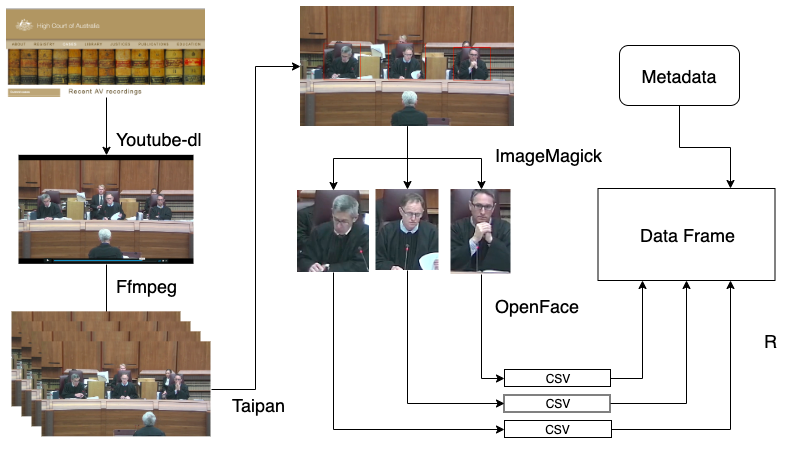
\includegraphics[width=1\linewidth]{figures/workflow} 

}

\caption{An illustration of the workflow for extracting facial variables from videos. \label{fig:workflow}}\label{fig:unnamed-chunk-1}
\end{figure}

\hypertarget{facial-variables-and-action-unit}{%
\section{Facial variables and action unit}\label{facial-variables-and-action-unit}}

OpenFace provides more than 711 variables measuring different aspects of a given face, a full description of the output variables can be found in \textcite{baltrusaitis2018openface}. The facial variables can be summarised into the following categories.

\begin{itemize}
\tightlist
\item
  \textbf{Confidence}: How confident OpenFace is in the detection.
\item
  \textbf{Gaze}: the vector from the pupil to corneal reflection. The dataset contains information on the gaze for both eyes with no distinct difference between the eyes.
\item
  \textbf{Pose}: the location of the head with respect to camera.
\item
  \textbf{Landmarking}: the location of certain characteristic points on the face and around the eyes. An illustration of face landmarks can be found in Figure \ref{fig:landmarking} in the Appendix.
\item
  \textbf{Action Unit}: An action unit is used to describe the movement of a single facial muscle.
\end{itemize}

The human facial expression can be de-constructed into a combination of action units. For example, happiness is the addition of action unit 6 and 12, which can be described as a raising check and a pull on the lip corner respectively. The Facial Action Coding System (FACS) is the common standard for describing facial expressions via anatomically decomposing a emotion into action units. To decompose an emotion of sadness, three action units are utilised. Action unit 01 describes the raise of inner brow; action unit 04 describes the general lower of brow and action unit 15 depicts the lower of lip corner. The subset of action units OpenFace is able to recognise is provided in Table \ref{tab:au} in the Appendix, along with their meaning and related emotions.

\hypertarget{data-format}{%
\section{Data format}\label{data-format}}

The data can be expressed in the long format with action unit as an index and presence and intensity presented as observations in two columns. Table \ref{tab:long} presents the data for Justices Edelman in case McKell for all the action units in the first frame in a long format. Since the frame is cropped at one minute interval, the intensity and presence can also be viewed as time series and Figure \ref{fig:ts-plot} plots the action unit 1 of Justices Edelman in case McKell across time.

\begin{table}[ht]
\begin{center}
\caption{\label{tab:long} An illustration of the data format for Justices Edelman in case McKell for all the action units in the first frame in long format.}
\begin{tabular}{lllllll}
\toprule
judge & video & frame & speaker & AU & presence & intensity \\
\midrule
Edelman & McKell & 1 & Appellent & AU01 & 0 & 0.05 \\
Edelman & McKell & 1 & Appellent & AU02 & 0 & 0.00 \\
Edelman & McKell & 1 & Appellent & AU04 & 0 & 0.01 \\
Edelman & McKell & 1 & Appellent & AU05 & 0 & 0.00 \\
Edelman & McKell & 1 & Appellent & AU06 & 0 & 0.00 \\
Edelman & McKell & 1 & Appellent & AU07 & 0 & 0.00 \\
Edelman & McKell & 1 & Appellent & AU09 & 0 & 0.26 \\
Edelman & McKell & 1 & Appellent & AU10 & 0 & 0.00 \\
Edelman & McKell & 1 & Appellent & AU12 & 0 & 0.00 \\
Edelman & McKell & 1 & Appellent & AU14 & 1 & 1.23 \\
Edelman & McKell & 1 & Appellent & AU15 & 0 & 0.46 \\
Edelman & McKell & 1 & Appellent & AU17 & 0 & 0.66 \\
Edelman & McKell & 1 & Appellent & AU20 & 1 & 1.44 \\
Edelman & McKell & 1 & Appellent & AU23 & 0 & 0.64 \\
Edelman & McKell & 1 & Appellent & AU25 & 0 & 0.00 \\
Edelman & McKell & 1 & Appellent & AU26 & 0 & 0.00 \\
Edelman & McKell & 1 & Appellent & AU45 & 0 & 0.25 \\
\bottomrule
\end{tabular}
\end{center}
\end{table}

\begin{figure}

{\centering 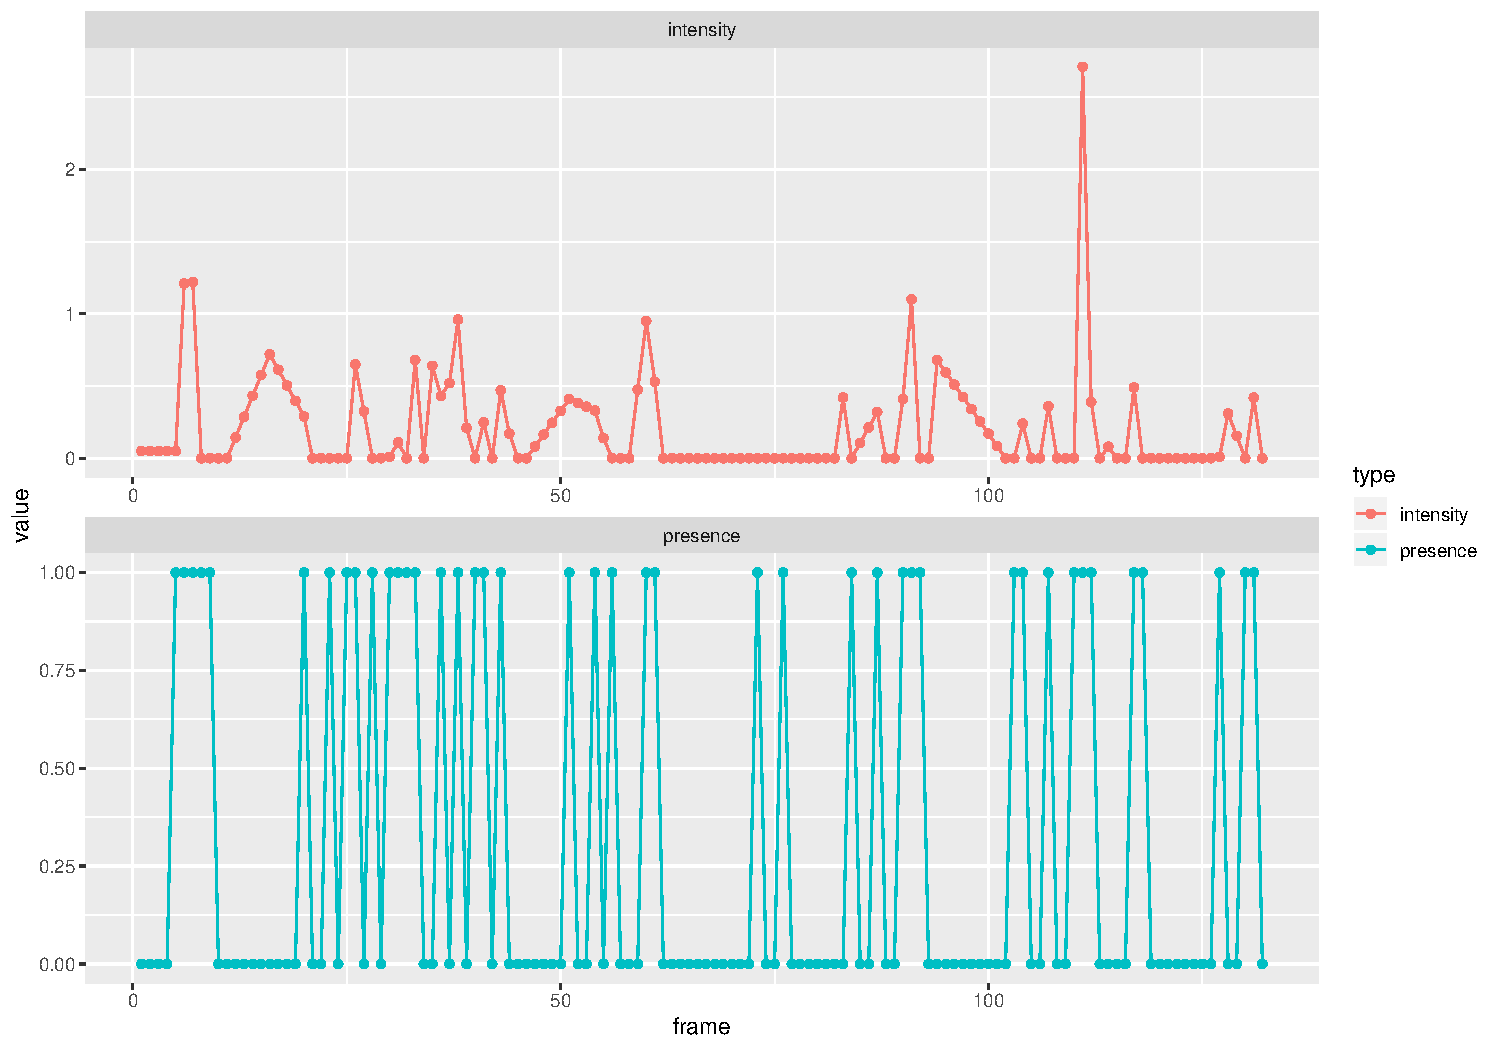
\includegraphics[width=1\linewidth]{figures/ts-plot-1} 

}

\caption{The intensity and presence score of action unit 01 for Justices Edelman in case McKell is graphed against time (frame number) as line chart. The intensity is a numerical variable while presence is binary variable takes value of 0 when the action uit is not present and 1 otherwise.}\label{fig:ts-plot}
\end{figure}

\hypertarget{missing-value-imputation}{%
\section{Missing value imputation}\label{missing-value-imputation}}

Missing values occur in the data whenever the justice is not looking straight ahead. This might occur when they are reading materials on their desk, or perhaps if conversing with their legal assistant behind them. It can also occur when there are five judges on a case, and the video resolution is not sufficiently high to detect the face or action units. The data structure that we created specifically places an NA in these positions. This has allowed us to examine the pattern of missings and check it happens more often in some recognisable way, for example when an appellant is speaking. We did not find any over-arching pattern, and thus have used a simple procedure to impute missings for intensity, which was then used to impute presence.

Intensity is a continuous variable ranging from zero or five measuring how strong the action unit is presented. The missing values of intensity are related to missing values in presence. Intensity being zero means the action unit is not present, being one means the action unit is present at minimum intensity and being five means the action unit is present at maximum intensity. Linear interpolation function (\texttt{na.interp()}) from \texttt{forecast} package is used to impute Intensity. The missing value of presence is then imputed based on if the intensity score of the missing observations are greater than one.

\hypertarget{source-code}{%
\section{Source code}\label{source-code}}

Source code for this data pre-processing is available at \url{https://github.com/huizezhang-sherry/ETC4860/data_pre_processing}.

\let\cleardoublepage\clearpage

\hypertarget{Ch:method}{%
\chapter{Methodology}\label{Ch:method}}

\hypertarget{notation}{%
\section{Notation}\label{notation}}

Let \(\mathbf{X}\) be a matrix of predictors, and \(\mathbf{Y}\) variable in our case is bivariate matrix of response variables, including a binary indicator of presence/absence and a numeric value measuring intensity, of facial action unit, where

\begin{itemize}
\tightlist
\item
  \(X_1\) indicates \texttt{judge} with six categories \(i = 1,2, \cdots, 6\)
\item
  \(X_2\) indicates \texttt{video} for each of the seven cases, \(j = 1,2, \cdots, 7\)
\item
  \(X_3\) indicates action unit containing 18 possible facial expression.
\item
  \(X_4\) indicates \texttt{speaker}, either the appellant or respondent, \(l=1,2\)
\item
  \(X_5\) indicates \texttt{frame} corresponding to time, \(t = 1,2, \cdots, T_j\)
\end{itemize}

Note that \(t\) could be considered a time variable, but because images are taken at 1 minute intervals, temporal dependence is unlikely to exist. Rather this should be considered an independent observation.

A full, main effects model for the data might be expressed as:

\[Y_{ijklt} = \mu + \alpha_i + \beta_j + \gamma_k + \delta_l + \varepsilon_{ijklt}\]

\noindent Also, let \(P_{jitkl}\) represent the response variable presence, and \(I_{jitkl}\) represent the response variable intensity. This notation will be helpful for defining the plots and models explained in this section.

\hypertarget{modelling-presence}{%
\section{Modelling presence}\label{modelling-presence}}

\hypertarget{model-structure}{%
\subsection{Model structure}\label{model-structure}}

The presence score is a binary variable that is one when a particular action unit is observed and zero if not. This suggests using a logistic model and we implement this using the \texttt{glm()} function from base R. The link function of a matter of choice in the \texttt{glm()} function and the logit link is chosen because it is the canonical link of the binomial family. An alternative link could be a probit link but theoretically, these two links give very similar result in terms of prediction \autocite{faraway2016extending}. The structure of the model is written as in Equation \ref{eq:logit-structure} with the first equation linking the mean of the presence to the linear prediction and the second equation specifying the linkage between \(\eta\) to the predictors. The next section will specify three different function form of the linear predictor by introducing different variables and interactions.

\begin{align}\label{eq:logit-structure}
\mu &= \frac{e^{\eta}}{1 + e^{\eta}} \\
\eta &= f(\alpha_i\text{,}\beta_j\text{,}\gamma_k\text{,}\delta_l)
\end{align}

\hypertarget{model-1-action-unit}{%
\subsection{Model 1: Action unit}\label{model-1-action-unit}}

The first linear function is written in Equation \ref{eq:judge_au}. It includes the main effect of judge and action unit and also their interaction. Interaction terms are included to capture the judge-wise differences for different action units and it is necessary because we suspect different judges could have different average presence scores for different action units.

\begin{align}\label{eq:judge_au}
\eta_{ik} &= \mu + \alpha_i + \gamma_k + (\alpha\gamma)_{ik}
\end{align}

\hypertarget{model-2-video}{%
\subsection{Model 2: Video}\label{model-2-video}}

Build upon the first model, the second model adds the video related main effect and interactions, as shown in Equation \ref{eq:judge_video}. The interactions allow both judge and action unit variables to differ in different videos, which is useful to answer the research questions \emph{whether the judges are behaving same or different across videos}.

\begin{align}\label{eq:judge_video}
\eta_{ijk} &= \mu + \alpha_i + \beta_j +\gamma_k + (\alpha\beta)_{ij} + (\alpha\gamma)_{ik} + (\beta\gamma)_{jk}
\end{align}

\noindent 

\hypertarget{model-3-speaker}{%
\subsection{Model 3: Speaker}\label{model-3-speaker}}

Build upon the second model, the third model is aimed to capture the speaker-wise effect by including the judge and speaker interaction as in Equation \ref{eq:judge_speaker}. This model would be helpful to answer the question \emph{do the expressions of the judges change when different parties are speaking}. The reason for not including more interaction between speaker and video or action unit is because this could cause the model to run out of degree of freedom given the number of observations we have.

\begin{align}\label{eq:judge_speaker}
\eta_{ijkl} &= \mu + \alpha_i + \beta_j +\gamma_k + \delta_l + (\alpha\beta)_{ij} + (\alpha\gamma)_{ik} + (\beta\gamma)_{jk} + (\alpha\delta)_{il}
\end{align}

\hypertarget{model-comparison}{%
\subsection{Model comparison}\label{model-comparison}}

The analysis of variance (ANOVA) \autocites{faraway2016extending}{gelman2006data} is a statistical method that can be used to compare different models. Different packages in R conduct ANOVA test: \texttt{anova()} and \texttt{drop()} from base R, \texttt{Anova()} from \texttt{car} package and \texttt{aov()} from \texttt{stats} package. We use the base R \texttt{anova()} function to compare the three models via chi-square tests.

\hypertarget{modelling-intensity}{%
\section{Modelling intensity}\label{modelling-intensity}}

The intensity score is a continuous variable, with 0 indicating an action unit is not present to a maximum intensity of 5. A histogram of the intensity is plotted in Figure \ref{fig:intensity} and the distribution has a high proportion of zeros with highly skewed continuous value. This type of data is the so-called semi-continuous data \autocite{twopart2010}. The semi-continuous data can be modelled in the econometrics literature by the two part model \autocite{cragg1971some}. In the two part model, the data is viewed to be generated via a sequential modelling technique, which is a mixed distribution of

\begin{itemize}
\tightlist
\item
  a logistic model of if Y = 0 or not, and
\item
  a specific model for the conditional distribution of \(y \mid y > 0\).
\end{itemize}

\begin{figure}

{\centering 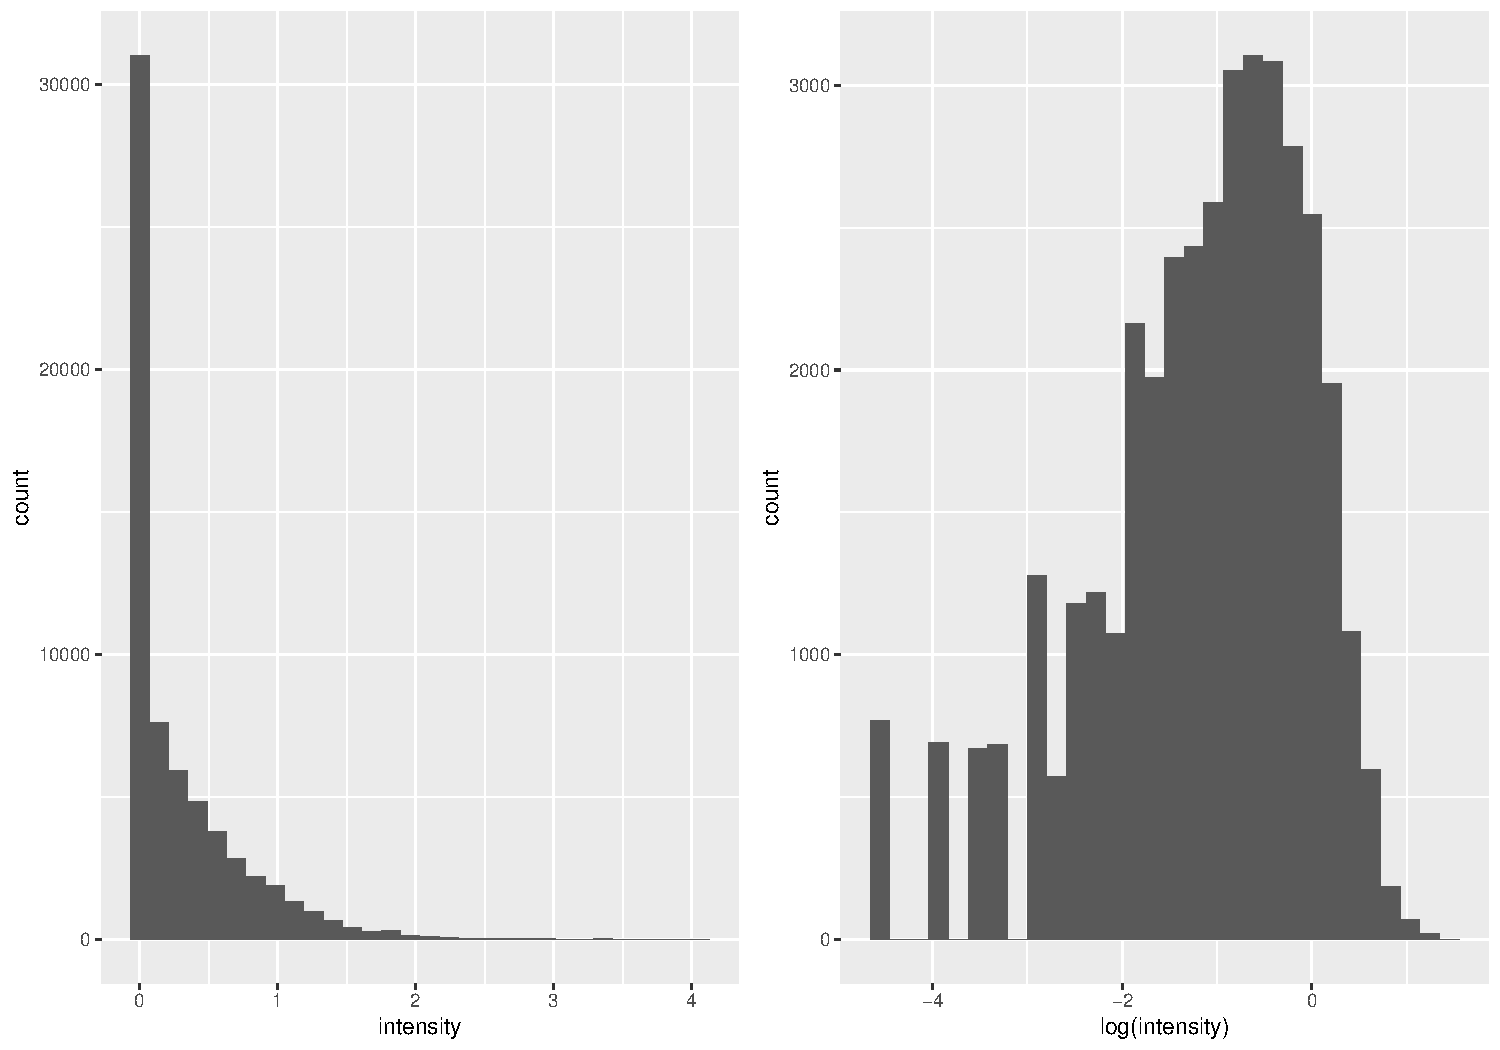
\includegraphics[width=1\linewidth]{figures/intensity-1} 

}

\caption{From the histogram of the intensity score, the data is highly skewed with an excessive amount of zeros. The two part model is about to accommodate the excessive zeros via the logistic model and gamma regression is about to capture the skewness in the data.}\label{fig:intensity}
\end{figure}

The choice of model between two part model and sample selection model is always discussed in the literature. Monte-Carlo simulation studies by different researchers \autocites{leung1996choice}{duan1984choosing}{manning1987monte} show different results on whether these different classes of model are answering the same or distinct inferential questions. The reason for us to choose two part model rather than sample selection model is because the problem of not being able to observe \(Y\) for those observations with selection variable \(z = 0\) doesn't exist in our data. In another word, if an action unit is not present for an observation, it doesn't make sense to talk about ``intensity score if the action unit is present''. Tobit model is not appropriate because the data can't be viewed as normally distributed with negative value censored as zero (meaningless to say negative intensity value). Zero inflated model is not used because it considers two source of zeros in the data while there is no zeros being generated from the second model (only one source of zeros).

The two part model has a general structure as in Equation \ref{eq:two-part-general}.

\begin{align}\label{eq:two-part-general}
\mu^1 &= \frac{e^{\eta}}{1 + e^{\eta}} \\
\eta &= f(\alpha_i, \beta_j, \gamma_k, \delta_l) \\
\mu^2 &= \log(I) \\
E(I \mid I > 0) &= f(\alpha_i, \beta_j, \gamma_k, \delta_l)
\end{align}

\noindent The first two equations capture the logistic link and its linear predictor. The next two specify the functional form of the conditional distribution. The functional form of the conditional distribution need to be able to capture the highly skewed nature of the non-zero observations. A convention approach is to assume the conditional distribution is a lognormal distribution \autocites{manning1981two}{diehr1999methods}. More recent literature proposes the use of gamma or generalised gamma regression model for the conditional distribution \autocite{twopart2010}. Gamma regression is used to because it could also capture the right skewness and it is easier to implement via the \texttt{glm()} function. The log link function is used because the canonical inverse link for gamma distribution will cause some estimated marginal mean to be extremely high and thus meaningless for intensity score.

The linear predictor of the conditional intensity that includes video and relevant interactions is written in Equation \ref{eq:two-part1}.

\begin{align}\label{eq:two-part1}
E(I_{ijk} \mid I_{ijk} > 0) &= \mu + \alpha_i + \beta_j +\gamma_k + (\alpha\beta)_{ij} + (\alpha\gamma)_{ik} + (\beta\gamma)_{jk}
\end{align}

The model that captures additional speaker variable is written in Equation \ref{eq:two-part2}.

\begin{align}\label{eq:two-part2}
E(I_{ijkl} \mid I_{ijkl} > 0) &= \mu + \alpha_i + \beta_j +\gamma_k + \delta_l + (\alpha\beta)_{ij} + (\alpha\gamma)_{ik} + (\beta\gamma)_{jk} + (\alpha\delta)_{il}
\end{align}

\hypertarget{post-model-analysis}{%
\section{Post-model analysis}\label{post-model-analysis}}

The estimates of variables from the model summary are not particularly useful in our case. This is because firstly, the estimates of the coefficient are not interpretable in the logistic regression. Secondly, we are interested in whether the mean for each treatment is same or different. To assess which level of the factor is different requires post-model analysis.

\hypertarget{estimated-marginal-mean-emm}{%
\subsection{Estimated Marginal Mean (EMM)}\label{estimated-marginal-mean-emm}}

The estimated marginal mean \autocite{gelman2006data} is the fitted value from a model over the treatment effects. In our data, the treatment effects include judge, video and action unit. The estimated marginal mean is computed using \texttt{emmean()} from the \texttt{emmenas} package. The probability from estimated marginal mean have a nice interpretation as the estimated probability of presence score for a particular combination of action unit, judge and video. This output allows us to compare how the estimated presence probabilities of each judge, video and action unit combination are different or similar from each other.

\hypertarget{confidence-interval-adjustment}{%
\subsection{Confidence Interval Adjustment}\label{confidence-interval-adjustment}}

The confidence intervals computed from the \texttt{emmean()} function need to be adjusted for simultaneous inference. A 5\% significance level indicates if we conduct 100 tests simultaneously, about 5 tests will show significance out of randomness. This is a problem we need to pay attention to when comparing the estimated presence probability or we may wrongly conclude judges has a different facial expression than others but they are actually not.

When multiple estimated mean are compared at the same time, the confidence level (or \(\alpha\) in p-value) need to be adjusted to control the family-wise error rate to be less than \(\alpha\). Bonferroni adjustment makes the adjustment to reject a hypothesis test at \(\alpha/N\) level so that the type I error of whole family of the simultaneous tests (Family-wise Error Rate (FWER)) is control be less than \(\alpha\). To do this, \texttt{confint()} function from base R is used with additional argument \texttt{adjust\ =\ "bonferroni"}.

\let\cleardoublepage\clearpage

\hypertarget{results}{%
\chapter{Results}\label{results}}

\hypertarget{exploratory-data-analysis}{%
\section{Exploratory data analysis}\label{exploratory-data-analysis}}

\hypertarget{action-unit-presence}{%
\subsection{Action unit: presence}\label{action-unit-presence}}

\hypertarget{mean-presence-score-and-most-common-action-units}{%
\subsubsection{Mean presence score and most common action units}\label{mean-presence-score-and-most-common-action-units}}

Follow the notation defined in section \ref{Ch:method}, the average presence score (\(P_{ik}\)) of each action unit is computed for each judge as \[P_{ik} = \frac{\sum_{jt}X_{ijtk}}{\sum_{j = 1}^JT_j}\]

\noindent Figure \ref{fig:mean_presence} graphs the presence score of all the action units across all the judges. The order of action unit on the y axis is ranked by the average presence of all the judges. The five most frequent action units are highlighted in blue. From Figure \ref{fig:mean_presence}, some of the action units are common across almost most of the Justices, these includes AU02 (outer eyebrow raiser), AU20 (lip stretcher), AU15 (lip corner depressor), AU01 (inner brow raiser) and AU14 (dimpler). Relating to emotions, AU01 and AU15 contribute to sadness. AU02, outer eyebrow raising can be associated with surprise, fear or interested. Dimpler (AU14) could be linked to contempt or boredom and Action unit 20, Lip Stretcher, is commonly contribute to fear, which is most sophisticated emotion that requires seven separate action units to describe.

\begin{figure}

{\centering 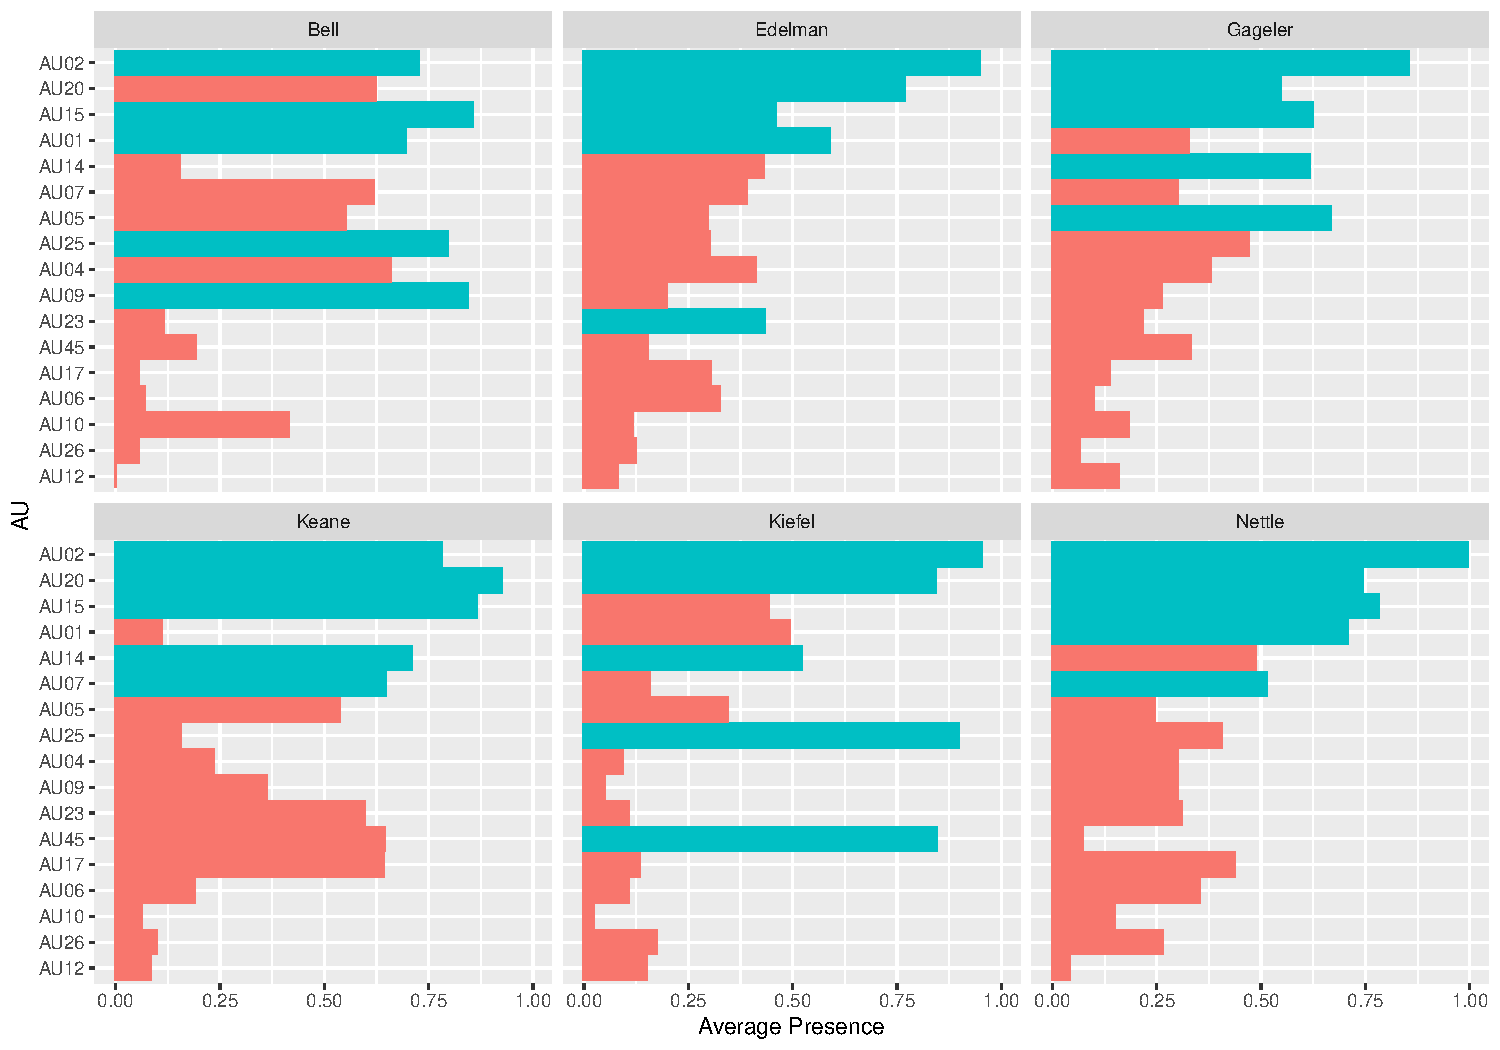
\includegraphics[width=1\linewidth]{figures/most-common-1} 

}

\caption{The average presence score of each action unit for each Justice, aggregating on video and time. The most common five action units for each Justices is colored in blue. The most common action units across all the Justices include AU02 (outer eyebrow raise), AU20 (lip stretcher), AU15 (Lip Corner Depressor), AU01 (Inner brow raise) and AU14 (Dimpler) \label{fig:mean_presence}}\label{fig:most-common}
\end{figure}

\hypertarget{presence-by-videos}{%
\subsubsection{Presence by videos}\label{presence-by-videos}}

The main presence score of the judges by video (\(P_{ijk}\)) is computed as \[P_{ijk} = \frac{\sum_{t}X_{ijtk}}{T_j}\] for the four most common action units: AU02, AU14, AU15, AU20 and presented in Figure \ref{fig:common_video}. From this figure, AU02, outer eyebrow raise, appears consistently highly across Justices and court cases. The other three vary across both Justices and cases. AU15, lip corner depressor, varies across Justices: it is common in Justices Bell, Keane and Nettle, but less common in Justices Keane and Edelman. Justice Gageler varies a lot in usage across cases and particularly uses this expression in OKS. AU20, lip stretcher is consistent across cases, varies by Justices, but is particularly frequently used in the OKS case by Justices Bell and Gageler. AU14, dimpler, is similar to AU20. Most reactions appear to be happening in case OKS and McKell. Recall that OKS is a criminal case involving misconduct with children, the result above provides some exploratory evidence that the Justices react more frequently in criminal cases like OKS and McKell.

\begin{figure}

{\centering 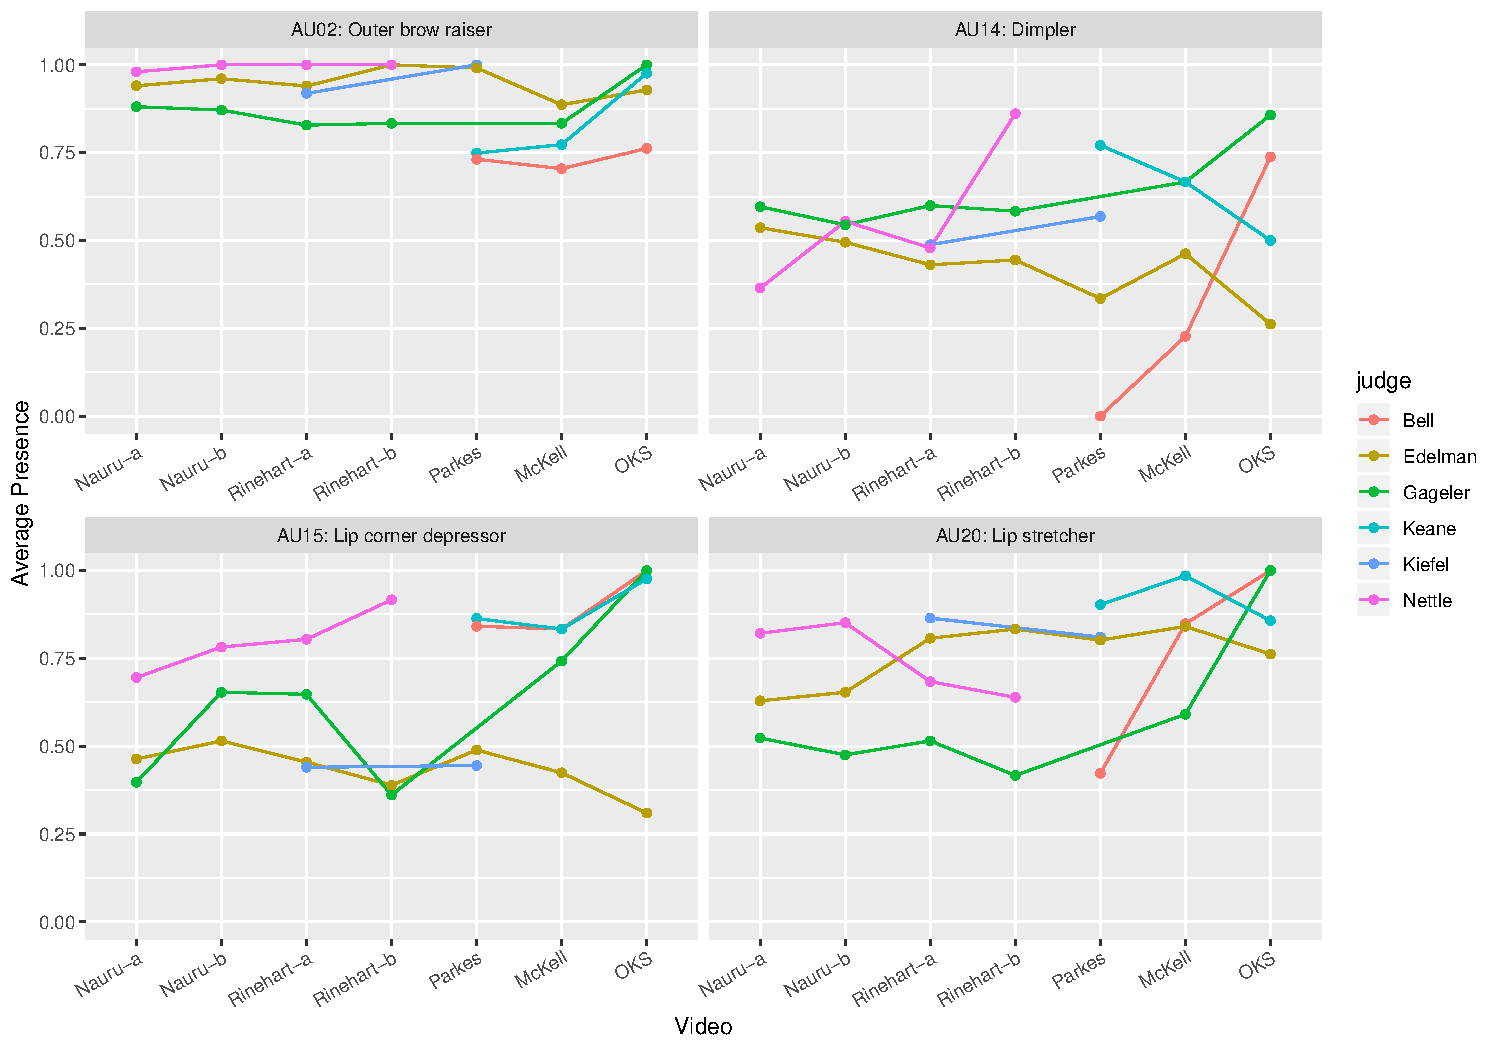
\includegraphics[width=1\linewidth]{figures/au-video-1} 

}

\caption{Average presence of the four most common action units for each judge by videos. Some Justices, for example Justices Gageler and Bell show large fluctuation on their facial expressions while others are not. \label{fig:common_video}}\label{fig:au-video}
\end{figure}

\hypertarget{action-unit-intensity}{%
\subsection{Action unit: intensity}\label{action-unit-intensity}}

\hypertarget{general-intensity-plot}{%
\subsubsection{General intensity plot}\label{general-intensity-plot}}

The boxplot of the intensity for all the Justices across all the videos is presented in Figure \ref{fig:intensity}. Each bar-and-whisker represents the intensity (\(I_{ijtk}\)) of all the action units aggregated on time for a particular Justices \(i\) in a specific case \(j\). For example, the first bar-and-whisker in case Nauru\_a is created using all the action units of Edelman through out the elapsed time in Nauru\_a case. The square root transformation is applied so that the mean of the intensity can be easier to visualise. Most of the action units have low intensity score as shown in the figure, which matches with the prior belief that the Justices are expected not to express to much of their expressions in the court room. Justices Nettle, colored in pink has the highest average in all the four cases he appeared.

\begin{figure}

{\centering 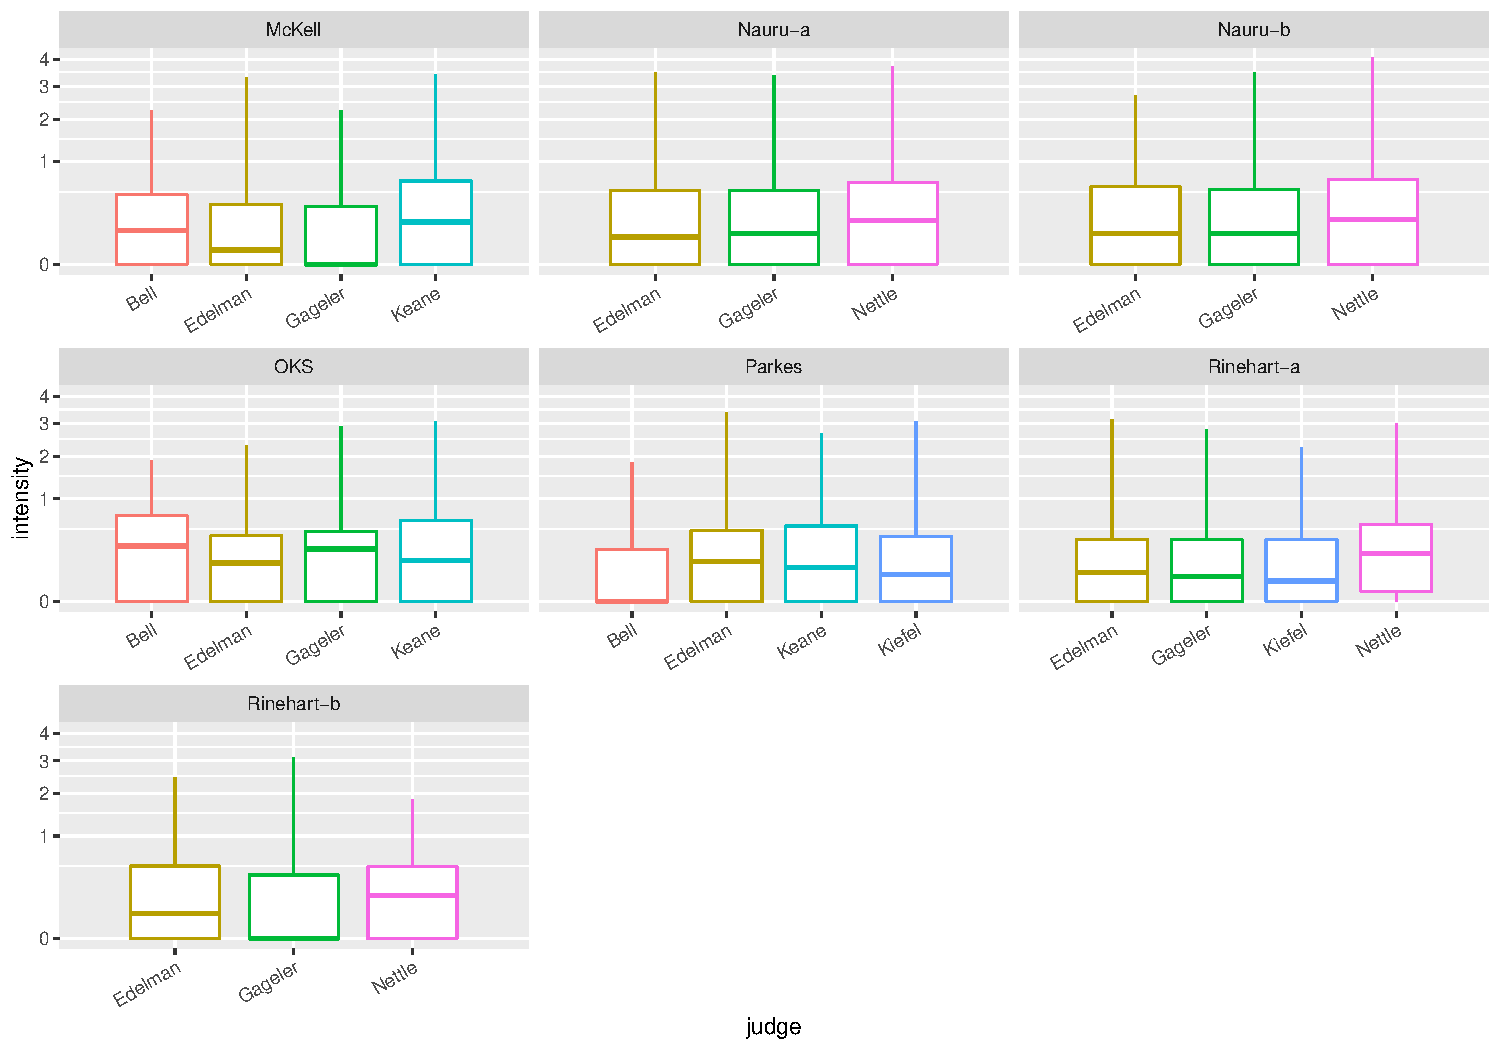
\includegraphics[width=1\linewidth]{figures/intensity-boxplot-1} 

}

\caption{Boxplot of intensity score by Justices and videos. Square root transformation is taken since the mean intensity scores are all below one.  \label{fig:intensity}}\label{fig:intensity-boxplot}
\end{figure}

\hypertarget{high-intensity-points}{%
\subsubsection{High intensity points}\label{high-intensity-points}}

The points with intensity greater than two are shown against time for all the justices in Figure \ref{fig:high-intensity-points}. Justices Edelman, Gageler and Nettle are the judges have stronger emotion that can be detected since they have more points with intensity greater than two. Different Justices also have different time where they display stronger emotions. For example, Justice Edelman are more likely to have stronger emotion throughout the time while Justices Nettle is more likely to have intense facial expressions at the beginning and ending of the hearing.

\begin{figure}

{\centering 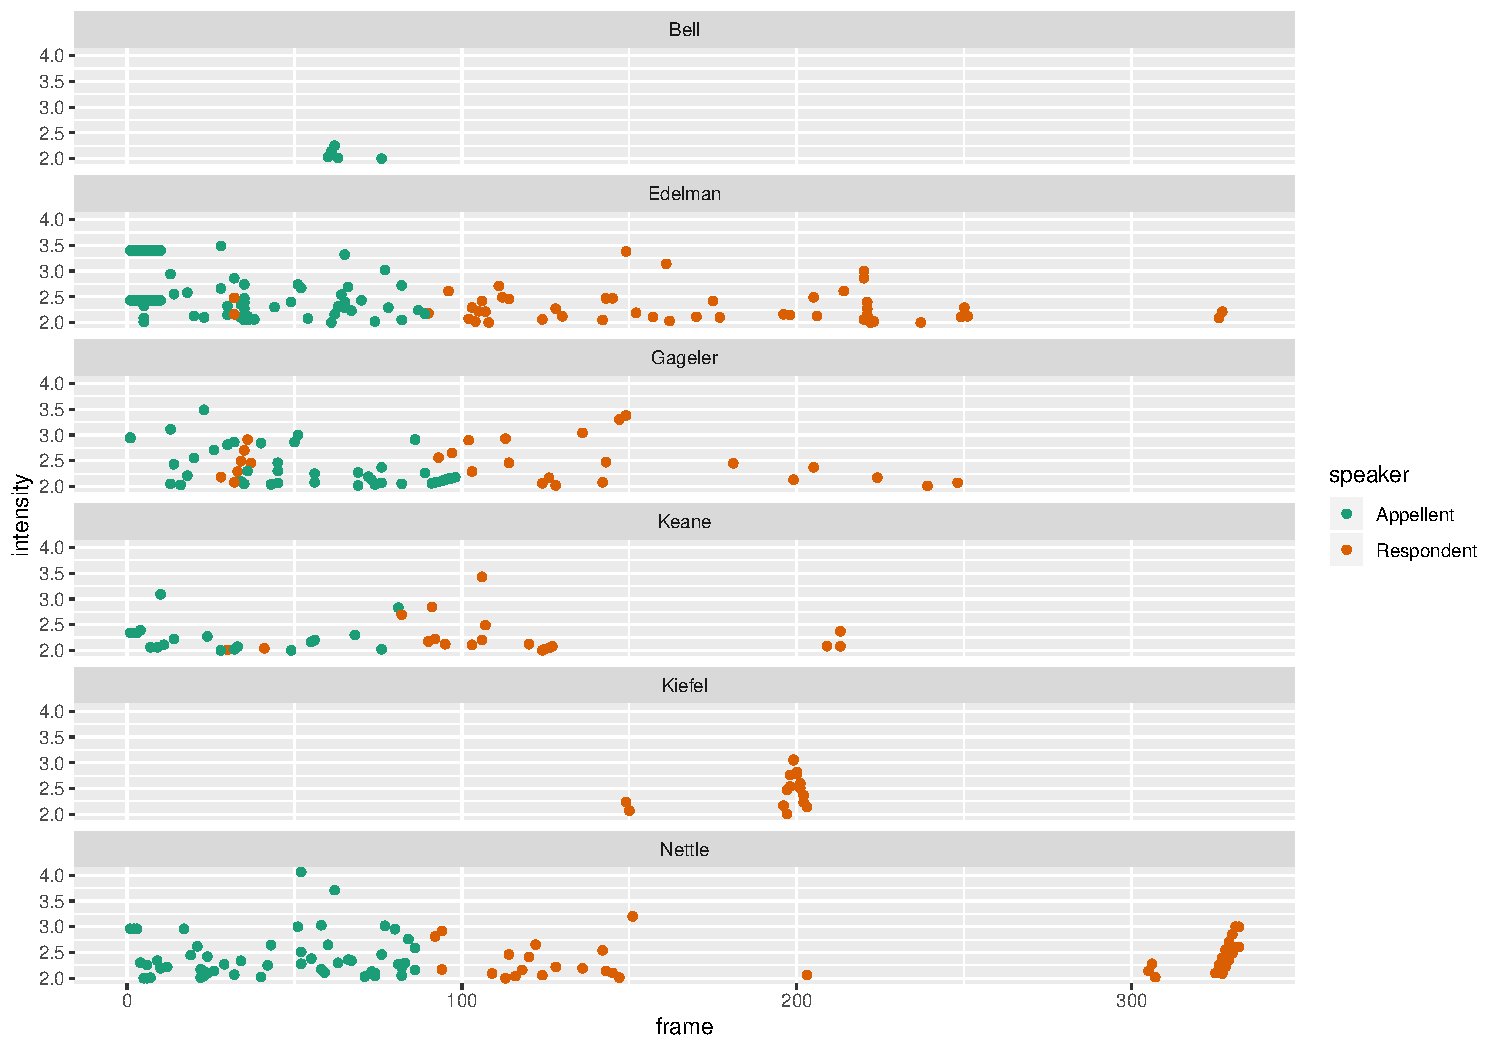
\includegraphics[width=1\linewidth]{figures/high-intensity-points-1} 

}

\caption{Points with intensity greater than two are plotted against time, colored by speaking parties. Justices Edelman, Gageler and Nettle have more intense expressions than other Justices. Justice Nettle has a clear cut on when he is likely to express stronger expressions. }\label{fig:high-intensity-points}
\end{figure}

\newpage

\hypertarget{summary}{%
\subsection{Summary}\label{summary}}

The findings from the exploratory data analysis are summarised below

\begin{itemize}
\item
  The most common action unit from the Justices are AU02 (outer eyebrow raiser), AU20 (lip stretcher), AU15 (lip corner depressor) and AU14 (dimpler).
\item
  Some Justices show relatively consistent facial expression through different videos while others, for example Justices Gageler and Bell have larger fluctuation on their facial expressions in different cases.
\item
  The overall intensity of the action units are low while Justices Nettle seems to have a relatively higher intensity than other Justices.
\item
  Edelman, Gageler and Nettle are the Justices with more intense facial expressions in the courtroom and Justices Nettle is the only Justice that tends to have stronger expression towards the end of the hearing.
\end{itemize}

\let\cleardoublepage\clearpage

\hypertarget{filtering-action-units}{%
\section{Filtering action units}\label{filtering-action-units}}

The number of action unit to include in the model is a matter of choice. The discussion of this choice is to ensure the model is parsimonious, that is, a model has the smallest number of variables but with greatest explanatory power. Random effect is a way to deal with large number of factor levels of a variable, but in our context, we are only interested in the action units with a certain mean presence and intensity for most of the judges.

The mean presence and intensity score for each action unit is computed and the action units to include in the model are the ones that appear in the top 10 action unit in both mean presence and intensity rank. This ensures that these action units have both relatively high intensity and presence score. A list of included action units along with their meaning and related emotions are presented in Table \ref{tab:au-included}

\begin{table}[ht]
\begin{center}
\caption{\label{tab:au-included} These are the selected action units that will be included in the modelling for intensity and presence.}
\begin{tabular}{lll}
\toprule
AU-number & meaning & emotion \\
\midrule
AU01 & Inner brow raiser & sadness, surprise and fear \\
AU04 & Brow lowerer & sadness, fear, anger and confusion \\
AU05 & Upper lid raiser & surprise, fear, anger adn interested \\
AU07 & Lid tightener & fear, anger and confusion \\
AU14 & Dimpler & contempt or boredom if appears unilateraly \\
AU15 & Lip corner depressor & sadness, disgust and confusion \\
AU20 & Lip stretcher & fear \\
AU45 & Blink & NA \\
\bottomrule
\end{tabular}
\end{center}
\end{table}

\hypertarget{modelling-result-for-presence}{%
\section{Modelling result for presence}\label{modelling-result-for-presence}}

\hypertarget{model-comparison-1}{%
\subsection{Model comparison}\label{model-comparison-1}}

The three models in Equation \ref{eq:judge_au}, \ref{eq:judge_video} and \ref{eq:judge_speaker} have been fitted and ANOVA test is performed to choose the best model. The ANOVA result for comparing Model 1 and 2 is presented in Table \ref{tab:anova-1}. After incorporating the main effect of case and its interaction with judge in Model 2, the degree of freedom is reduced by 61. This has a significant improvement on the model since the p-value (1e-88) is close to zero, indicating the null hypothesis that Model 1 and Model 2 are the same is rejected.

The ANOVA result between Model 2 and Model 3 is presented in Table \ref{tab:anova-2}. The additional six variables associated with speakers in Model 3 have improved the model at 95\% significance level since the p-value (0.027) is less than 0.05, however, at 99\% significicance level, this improvement is not significant. Model 2 is chosen as the final model because the interpretation of video-wise effect using Model 2 after post-model analysis provides more interesting findings about the expressions of the Justices than the speaker-wise effect using Model 3.

\begin{table}[ht]
\begin{center}
\caption{\label{tab:anova-1}Model comparison using ANOVA for Model 1 and 2. The inclusion of video related variables in Model 2 decreases the degree of freedom by 61 while provides a significant improvement on the model as indicated by the p-value. }
\begin{tabular}{lrrlll}
\toprule
Model & Resid. Df & Resid. Dev & Df & Deviance & Pr(>Chi) \\
\midrule
Model 1 & 30320 & 35850.07 &   &   &   \\
Model 2 & 30259 & 35255.72 & 61 & 594 & 1.8e-88 \\
\bottomrule
\end{tabular}
\end{center}
\end{table}

\begin{table}[ht]
\begin{center}
\caption{\label{tab:anova-2}The model comparison result of Model 2 and Model 3 using ANOVA. The inclusion of six speaker related main and interaction effects contribute to improve the model. However, this is not significant at 99\% significant level. Model 2 is chosen as the final model because the interpretation of video effect provides more interesting findings about the facial expressions of the Justices. }
\begin{tabular}{lrrlll}
\toprule
Model & Resid. Df & Resid. Dev & Df & Deviance & Pr(>Chi) \\
\midrule
Model 2 & 30259 & 35255.72 &   &   &   \\
Model 3 & 30253 & 35241.51 & 6 & 14 & 0.027 \\
\bottomrule
\end{tabular}
\end{center}
\end{table}

\hypertarget{residual-diagnostics-and-post-model-analysis}{%
\subsection{Residual Diagnostics and post-model analysis}\label{residual-diagnostics-and-post-model-analysis}}

The residuals of Model 2 are plotted against variable judge and video in Figure \ref{fig:resid-judge} and \ref{fig:resid-video} in the Appendix. There is no obvious pattern shown in the residuals for different Justices or videos, which indicates adequate fit.

The estimated marginal mean is computed and presented in Table \ref{tab:result-2} in the Appendix due to its length. The \texttt{prob} column can be interpreted as after averaging over all the videos and speaking parties, the estimated mean probability for judge Edelman in action unit AU02 is 0.95, with a 95\% confidence interval of {[}0.92, 0.97{]}. Notice that confidence intervals for a generalised linear model is asymmetric around the estimates because the linear symmetric interval of the mean has been transferred via the inverse of link function to get the confidence interval for the response.

\hypertarget{the-presence-of-facial-expression-of-the-justices-by-video}{%
\subsection{The presence of facial expression of the justices by video}\label{the-presence-of-facial-expression-of-the-justices-by-video}}

The 95\% confidence interval after bonferroni adjustment is plotted in Figure \ref{fig:model2-plot}. In general, most of the intervals for the same judge in the same action unit are overlapping with each other on the vertical axis, while there are some non-overlappings highlight the potential inconsistency of the facial expressions of the Justices.

Justice Edelman and Keane behave consistently throughout all the videos, while they both seem to express significantly less in action unit 5 (upper lid raiser) in the OKS case. Justice Nettle has relatively low expression of action unit 4 (brow lowerer) in case Rinehart-a. Gageler shows a consistently high number of expressions in case OKS for action unit 15 (lip corner depressor) and action unit 20 (lip stretcher).

Bell presents similar reactions to Gageler, showing a significantly higher proportion of emotions associated with action unit 1 (inner brow raiser), 14 (dimpler), 15 (lip corner depressor) and 20 (lip stretcher) in case OKS. Bell also exhibits less presence of action unit 07 (lid tightener) and 20 (lip stretcher) in case Parkes.

\begin{figure}

{\centering 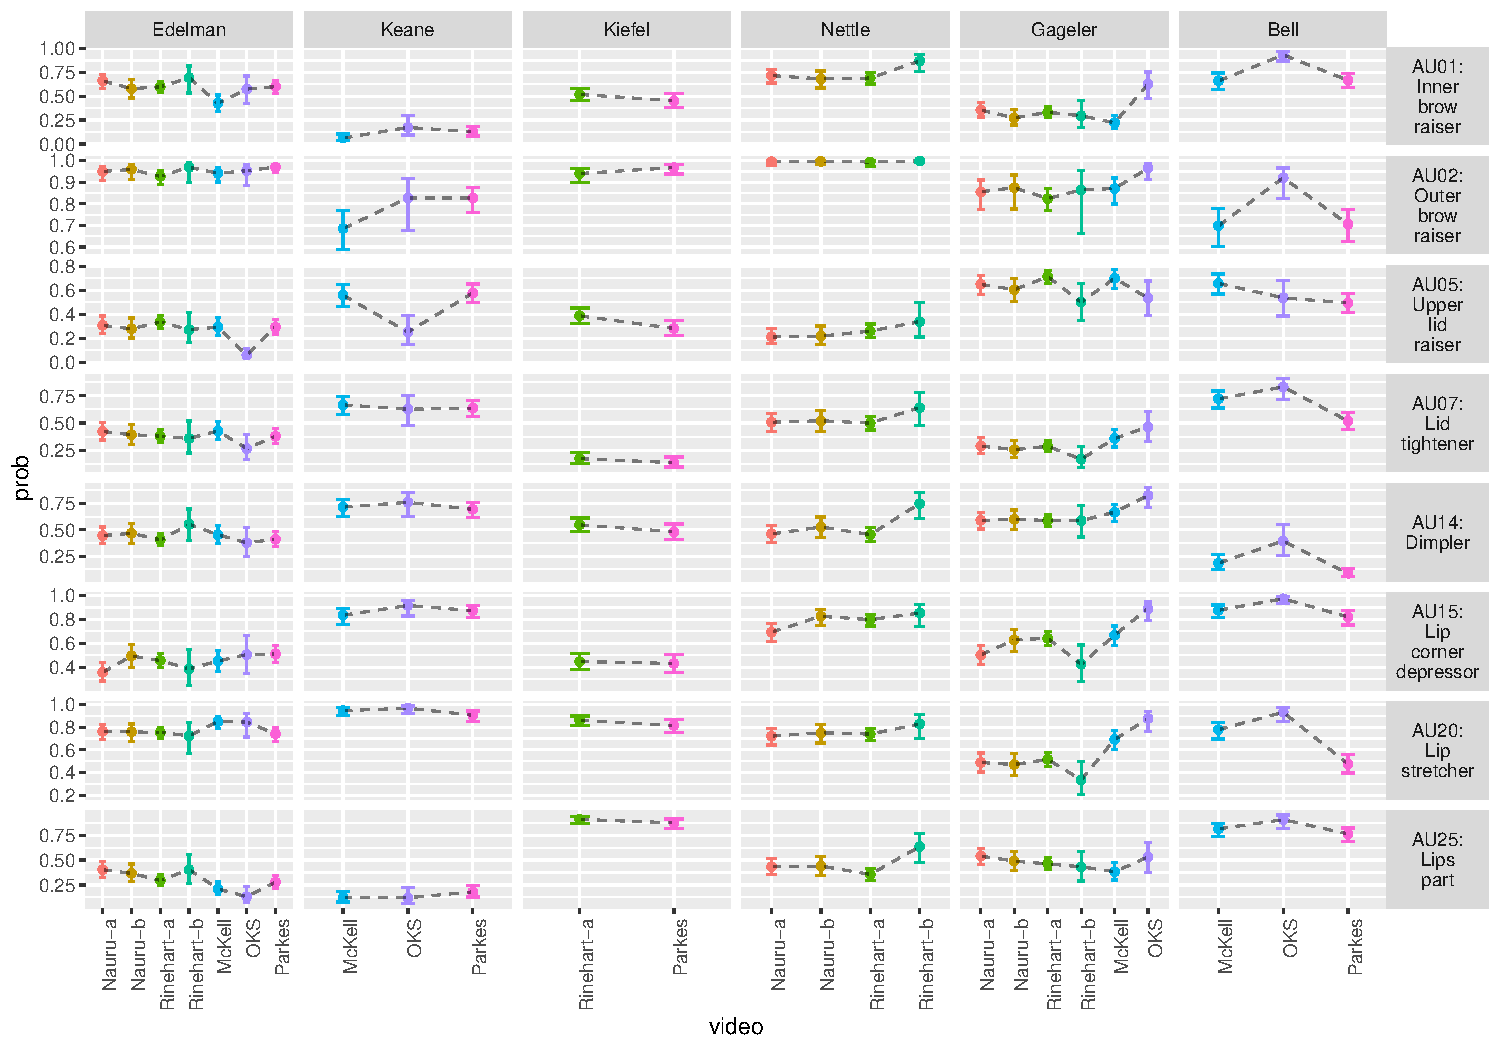
\includegraphics[width=1\linewidth]{figures/model2-plot-1} 

}

\caption{The 95\% confidence interval for estimated mearginal mean for presence after bonferroni adjustment. The x axis represents video and the y axis represents the estimated marginal mean of an action unit being observed. The facet shows the Justices in columns and action units in rows. }\label{fig:model2-plot}
\end{figure}

\hypertarget{modelling-result-for-intensity}{%
\section{Modelling result for intensity}\label{modelling-result-for-intensity}}

\hypertarget{the-intensity-of-facial-expression-of-the-justices-by-video}{%
\subsection{The intensity of facial expression of the justices by video}\label{the-intensity-of-facial-expression-of-the-justices-by-video}}

The two part model in equation \ref{eq:two-part1} is estimated for the intensity data. Estimated marginal mean and confidence interval adjustment procedure are performed as modelling presence data. The 95\% confidence interval plot is presented in Figure \ref{fig:intensity-video}. This shows that Justices Edelman has significantly stronger expressions of brow lowerer (AU04) in case Nauru-a, Nauru-b and Rinehart-a, but less intensity when expressing lid tightener (AU07) in case OKS. Justice Keane also shows more intense expressions of lid tightener (AU07) in case McKell.

Action unit 5 (upperlid raiser) and 20 (lip stretcher) are exhibited significantly more intense for Justices Gageler in case OKS. The mean for brow lowerer (AU04) seems to higher than those in other cases for Justices Gageler but this result is not significant.

For Justice Bell, the intensity of inner brow raiser (AU01), upper lid raiser (AU05), dimpler (AU14) and Lip stretcher (AU20) are also significantly higher in case OKS.

\begin{figure}

{\centering 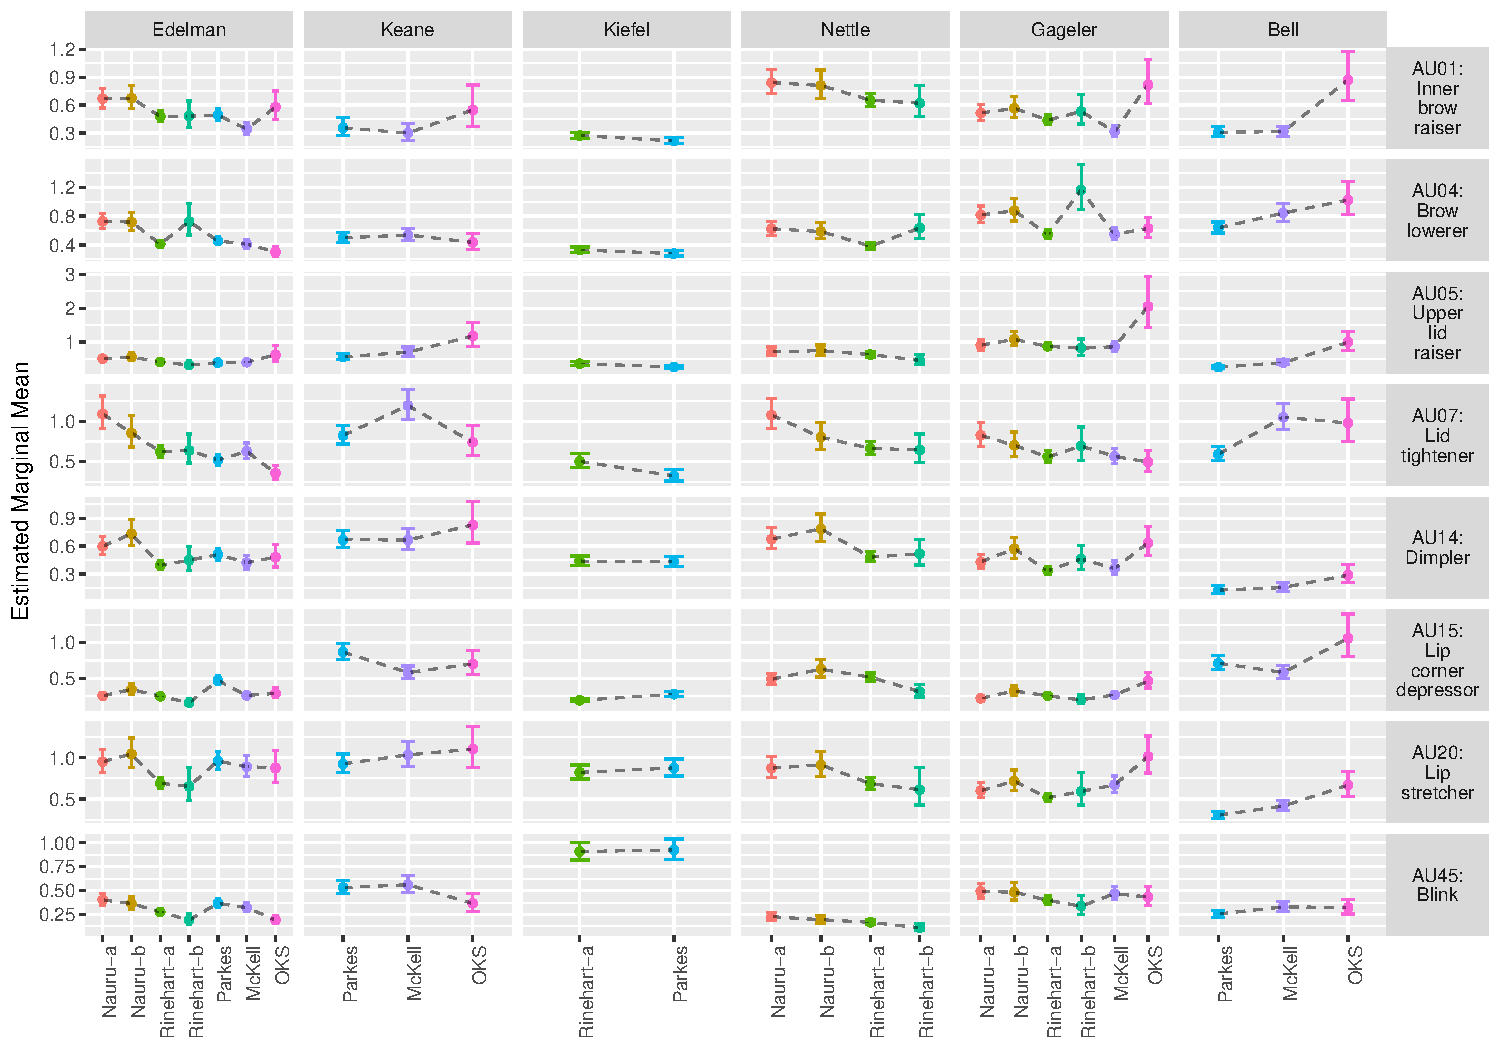
\includegraphics[width=1\linewidth]{figures/intensity-video-1} 

}

\caption{The 95\% confidence interval for estimated mearginal mean for presence after bonferroni adjustment. The x axis represents video and the y axis represents the estimated marginal mean of the intensity. The facet shows the Justices in columns and action units in rows. }\label{fig:intensity-video}
\end{figure}

\hypertarget{the-expression-of-the-justices-by-speaker}{%
\subsection{The expression of the justices by speaker}\label{the-expression-of-the-justices-by-speaker}}

From the presence and intensity figures which are colored by speakers in Figure \ref{fig:model3-plot} and \ref{fig:intensity-speaker} in the Appendix, we can observe that the video-wise difference between Justices is still preserved when the speaker effects are included in the model. However, the speaker-wise difference is not significant in terms of both presence and intensity for all the Justices.

\let\cleardoublepage\clearpage

\hypertarget{insights}{%
\section{Insights}\label{insights}}

This result from previous chapter contributes to answer the question: \textbf{For the same judge, does the mean presence and mean intensity of the action units stay the same or vary for different videos?} In general, the facial expressions of the justices appear impartial, as most of the 95\% confidence intervals for the same judge and action unit overlap in the vertical direction in most of the videos in both figures. There are some instances when in a particular video, a judge expressed significantly more or less of an expression.

It is necessary to link back to the nature of the cases to interpret the facial behaviour of the Justices. Nauru-a and Nauru-b discusses immigration law; McKell and OKS are more criminal cases; Parkes is a civil negligence case and Rinehart-a and Rinehart-b are commercial cases arguing contract arbitration.

Based on the nature of the cases, Justice Edelman is more likely to express stronger emotion to the immigration and commercial cases and express less and softer at criminal cases. The action unit 5 (upper lid raiser) and 7 (lid tightener), which are expressed more frequent and more intense by Justice Keane in case OKS are usually associated with the emotion of anger. This implies that Justices Keane is more responsive to the criminal cases. Kiefel and Nettle are relatively consistent in their expressions. Of the six universal emotions, the action units Justices Gageler have significantly more frequent and stronger in case OKS are action unit 5 (upper lid raiser), 15 (lip corner depressor) and 20 (lip stretcher). These three action units are commonly associated with anger, sadness and fear respectively, which indicate Justice Gageler's strong and frequent emotional responses when hearing criminal cases OKS. The result for Bell suggest the same emotional reaction as judge Gageler to criminal cases.

As the speaker-wise difference was not significant, suggestions that Justice favour an appellant or respondent were not confirmed. This result would be a validation that on the high court level, the judges are behaving impartial to different speaking parties.

To summarise, the above discussion of intensity and presence of action unit in different cases gives us several findings about the expression of the judges:

\begin{enumerate}
\def\labelenumi{\arabic{enumi})}
\item
  In general, the expression of the Justices are impartial, which is live up to the code of conduct from \textcite{judicalguid} and validate the result from \textcite{tutton2018judicial}.
\item
  When there is significantly present or intense expression of the Justices, it tends to be associated with negative emotion like sad, fear and anger. This could have implication on the mental well-being of the judges.
\item
  Some justices, for example Keane, Gageler and Bell are more responsive, both in frequency (mean presence) and magnitude (mean intensity) to criminal cases. This could show that it is harder for judges to keep a still face when the content of a case goes against human nature.
\end{enumerate}

\hypertarget{conclusion-limitation-and-future-work}{%
\chapter{Conclusion, limitation and future work}\label{conclusion-limitation-and-future-work}}

\hypertarget{conclusion}{%
\section{Conclusion}\label{conclusion}}

In this thesis, we explore the facial expressions of seven high court Justices in six cases utilising the publicly available videos from the high court hearing. The main aim of this research is to use a statistical and objective approach to understand whether the Justices are behaving impartial in the courtroom.

Our approach involves extracting facial variables from the videos of the high court hearings and statistically model the presence and intensity of the action units. This allows us to understand whether different Justices would have variations in their expressions in different cases and whether their expressions will be different when different parties are speaking. We have found that in general, the Justices are behaving impartial during the court, which is a validation on Tutton's ethnographic study on the same topic. We also find that Justices tend to have stronger and more frequent negative emotions, for example sad, anger and fear in criminal cases. From a humanity perspective, it could be hard for the Justices control their expressions in criminal cases when extreme and violent scenes are described in the hearing.

One of highlights of the project is to establish a workflow for systematically extracting facial variables from videos. The established workflow makes it easy for any re-processing of the videos and analysing facial expressions from other video source. Furthermore, as far as we know, this study is the first of its kind to statistically analyse videos to study the emotions in the courtroom. This piece of work therefore makes a significant contribution to the legal research by providing a new, statistical methodology to understand the emotion of the Justices. The facial information gained from this research could also be incorporated with other judicial information to predict the high court case outcome in Australia.

\hypertarget{limitation}{%
\section{Limitation}\label{limitation}}

The current image frames are extracted at every one minute interval. However, some facial expressions may only last for a few second. Thus more frequent time interval could be used for getting more precise facial information of the judges. Also, if videos of the high court hearing could be accepted as input for facial expression detection, the potential correlation of emotion could be captured even better.

In my work, seven videos are being processed into the facial recognition software and more videos could be processed to get more robust results. The reason for not processing more videos in the current study is because the resolution of publicly available videos from the high court has only 720 pixels while the facial recognition software, OpenFace requires at least 30 pixels for a face to be detected. This means that we have to choose videos where three or five judges are presented.

However, this work has established a workflow for extracting facial expressions of human from videos. As long as more higher resolution videos are available, facial variables can be extracted via the same fashion.

\hypertarget{future-work}{%
\section{Future work}\label{future-work}}

Faces could be extracted more often than at 1 minute intervals to allow researchers to capture more precise expressions of the judges. However, as the extraction becomes more frequent, the problem of serial correlation could rise and appropriate modelling technique should be utilised to accommodate for this feature of data.

\hypertarget{acknowledgement}{%
\section{Acknowledgement}\label{acknowledgement}}

The analysis is conducted using R \autocite{Rlanguage}, and the following packages: forecast \autocite{forecast}, tidyverse \autocite{tidyverse}, emmenas \autocite{emmeans} and broom \autocite{broom}. This thesis document is created with knitr \autocite{knitr}, R Markdown \autocite{rmarkdown} and bookdown \autocite{bookdown}. All matrials required to reproduce the project can be found at \url{https://github.com/huizezhang-sherry/ETC4860/}.

\hypertarget{appendix}{%
\chapter{Appendix}\label{appendix}}

\hypertarget{list-of-videos-used-in-the-project}{%
\section{List of videos used in the project}\label{list-of-videos-used-in-the-project}}

\begin{longtable}[]{@{}llll@{}}
\caption{Details of videos processed.}\tabularnewline
\toprule
\begin{minipage}[b]{0.22\columnwidth}\raggedright
Case\strut
\end{minipage} & \begin{minipage}[b]{0.15\columnwidth}\raggedright
Name\strut
\end{minipage} & \begin{minipage}[b]{0.30\columnwidth}\raggedright
AV recording link\strut
\end{minipage} & \begin{minipage}[b]{0.22\columnwidth}\raggedright
Judge\strut
\end{minipage}\tabularnewline
\midrule
\endfirsthead
\toprule
\begin{minipage}[b]{0.22\columnwidth}\raggedright
Case\strut
\end{minipage} & \begin{minipage}[b]{0.15\columnwidth}\raggedright
Name\strut
\end{minipage} & \begin{minipage}[b]{0.30\columnwidth}\raggedright
AV recording link\strut
\end{minipage} & \begin{minipage}[b]{0.22\columnwidth}\raggedright
Judge\strut
\end{minipage}\tabularnewline
\midrule
\endhead
\begin{minipage}[t]{0.22\columnwidth}\raggedright
The Republic of Nauru v WET040 {[}No.~2{]} {[}2018{]} HCA 60\strut
\end{minipage} & \begin{minipage}[t]{0.15\columnwidth}\raggedright
\texttt{Nauru\_a}\strut
\end{minipage} & \begin{minipage}[t]{0.30\columnwidth}\raggedright
\url{http://www.hcourt.gov.au/cases/cases-av/av-2018-11-07a}\strut
\end{minipage} & \begin{minipage}[t]{0.22\columnwidth}\raggedright
Nettle, Gageler, Edelman\strut
\end{minipage}\tabularnewline
\begin{minipage}[t]{0.22\columnwidth}\raggedright
TTY167 v Republic of Nauru {[}2018{]} HCA 61\strut
\end{minipage} & \begin{minipage}[t]{0.15\columnwidth}\raggedright
\texttt{Nauru\_b}\strut
\end{minipage} & \begin{minipage}[t]{0.30\columnwidth}\raggedright
\url{http://www.hcourt.gov.au/cases/cases-av/av-2018-11-07b}\strut
\end{minipage} & \begin{minipage}[t]{0.22\columnwidth}\raggedright
Nettle, Gageler, Edelman\strut
\end{minipage}\tabularnewline
\begin{minipage}[t]{0.22\columnwidth}\raggedright
Rinehart v Hancock Prospecting Pty Ltd {[}2019{]} HCA 13\strut
\end{minipage} & \begin{minipage}[t]{0.15\columnwidth}\raggedright
\texttt{Rinehart\_a}\strut
\end{minipage} & \begin{minipage}[t]{0.30\columnwidth}\raggedright
\url{http://www.hcourt.gov.au/cases/cases-av/av-2018-11-13}\strut
\end{minipage} & \begin{minipage}[t]{0.22\columnwidth}\raggedright
Gordon, Gageler, Bell, Keane, Edelman\strut
\end{minipage}\tabularnewline
\begin{minipage}[t]{0.22\columnwidth}\raggedright
Rinehart v Hancock Prospecting Pty Ltd {[}2019{]} HCA 13\strut
\end{minipage} & \begin{minipage}[t]{0.15\columnwidth}\raggedright
\texttt{Rinehart\_b}\strut
\end{minipage} & \begin{minipage}[t]{0.30\columnwidth}\raggedright
\url{http://www.hcourt.gov.au/cases/cases-av/av-2018-11-14a}\strut
\end{minipage} & \begin{minipage}[t]{0.22\columnwidth}\raggedright
Gordon, Keane, Bell, Gageler, Edelman\strut
\end{minipage}\tabularnewline
\begin{minipage}[t]{0.22\columnwidth}\raggedright
Parkes Shire Council v South West Helicopters Pty Limited {[}2019{]} HCA 14\strut
\end{minipage} & \begin{minipage}[t]{0.15\columnwidth}\raggedright
\texttt{Parkes}\strut
\end{minipage} & \begin{minipage}[t]{0.30\columnwidth}\raggedright
\url{http://www.hcourt.gov.au/cases/cases-av/av-2018-11-14b}\strut
\end{minipage} & \begin{minipage}[t]{0.22\columnwidth}\raggedright
Gordon, Bell, Kiefel, Keane, Edelman\strut
\end{minipage}\tabularnewline
\begin{minipage}[t]{0.22\columnwidth}\raggedright
McKell v The Queen {[}2019{]} HCA 5\strut
\end{minipage} & \begin{minipage}[t]{0.15\columnwidth}\raggedright
\texttt{McKell}\strut
\end{minipage} & \begin{minipage}[t]{0.30\columnwidth}\raggedright
\url{http://www.hcourt.gov.au/cases/cases-av/av-2018-12-07}\strut
\end{minipage} & \begin{minipage}[t]{0.22\columnwidth}\raggedright
Gordon, Gageler, Kiefel, Nettle, Edelman\strut
\end{minipage}\tabularnewline
\begin{minipage}[t]{0.22\columnwidth}\raggedright
OKS v Western Australia {[}2019{]} HCA 10\strut
\end{minipage} & \begin{minipage}[t]{0.15\columnwidth}\raggedright
\texttt{OKS}\strut
\end{minipage} & \begin{minipage}[t]{0.30\columnwidth}\raggedright
\url{http://www.hcourt.gov.au/cases/cases-av/av-2019-02-14}\strut
\end{minipage} & \begin{minipage}[t]{0.22\columnwidth}\raggedright
Gordon, Gageler, Kiefel, Nettle, Edelman\strut
\end{minipage}\tabularnewline
\bottomrule
\end{longtable}

\hypertarget{an-illustration-of-face-landmarking}{%
\section{An illustration of face landmarking}\label{an-illustration-of-face-landmarking}}

\begin{figure}

{\centering 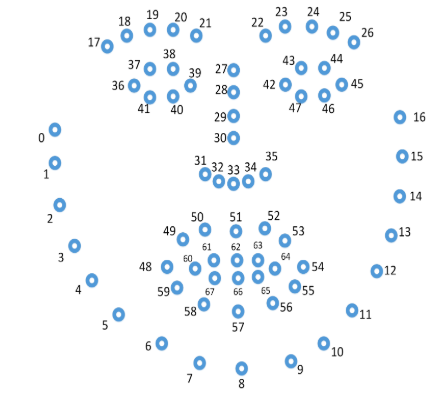
\includegraphics[width=1\linewidth]{figures/landmarking} 

}

\caption{An illustration of the face landmarking where 67 key points on a face is identified. OpenFace provides 2D and 3D coordinates of these landmarking points}\label{fig:landmarking}
\end{figure}

\hypertarget{description-of-action-units-recognised-by-openface}{%
\section{Description of action units recognised by OpenFace}\label{description-of-action-units-recognised-by-openface}}

\begin{table}[ht]
\begin{center}
\caption{\label{tab:au} The subset of action units OpenFace is able to recognise.}
\begin{tabular}{lll}
\toprule
AU-number & AU-meaning & emotion \\
\midrule
AU01 & AU01: Inner brow raiser & sadness, surprise and fear \\
AU02 & AU02: Outer brow raiser & surprise, fear and interested \\
AU04 & AU04: Brow lowerer & sadness, fear, anger and confusion \\
AU05 & AU05: Upper lid raiser & surprise, fear, anger adn interested \\
AU06 & AU06: Cheek raiser & happiness \\
AU07 & AU07: Lid tightener & fear, anger and confusion \\
AU09 & AU09: Nose wrinkler & disgust \\
AU10 & AU10: Upper lip raiser & NA \\
AU12 & AU12: Lip corner puller & happiness and possibly contempt if appears unilateraly \\
AU14 & AU14: Dimpler & contempt or boredom if appears unilateraly \\
AU15 & AU15: Lip corner depressor & sadness, disgust and confusion \\
AU17 & AU17: Chin raiser & interested and confusion \\
AU20 & AU20: Lip stretcher & fear \\
AU23 & AU23: Lip tightener & anger, confusion or bordom \\
AU25 & AU25: Lips part & NA \\
AU26 & AU26: Jaw drop & surprise and fear \\
AU28 & AU28: Lip suck & NA \\
AU45 & AU45: Blink & NA \\
\bottomrule
\end{tabular}
\end{center}
\end{table}

\hypertarget{model-estimation-result}{%
\section{Model estimation result}\label{model-estimation-result}}

\begin{center}
\begin{longtable}{lllllll}
\caption{\label{tab:result-2}Estimated marginal means of presence for model 2. }\\
\toprule
judge & video & AU & prob & SE & asymp.LCL & asymp.UCL \\
\midrule
\endhead
\bottomrule
\endfoot
Edelman & Nauru-a & AU01 & 0.678 & 0.0276 & 0.599 & 0.747 \\
Nettle & Nauru-a & AU01 & 0.721 & 0.0269 & 0.643 & 0.787 \\
Gageler & Nauru-a & AU01 & 0.337 & 0.0283 & 0.265 & 0.416 \\
Edelman & Nauru-b & AU01 & 0.589 & 0.0354 & 0.491 & 0.680 \\
Nettle & Nauru-b & AU01 & 0.673 & 0.0337 & 0.577 & 0.756 \\
Gageler & Nauru-b & AU01 & 0.273 & 0.0302 & 0.200 & 0.361 \\
Edelman & Rinehart-a & AU01 & 0.597 & 0.0212 & 0.539 & 0.652 \\
Kiefel & Rinehart-a & AU01 & 0.524 & 0.0245 & 0.458 & 0.589 \\
Nettle & Rinehart-a & AU01 & 0.697 & 0.0215 & 0.637 & 0.752 \\
Gageler & Rinehart-a & AU01 & 0.323 & 0.0208 & 0.270 & 0.382 \\
Edelman & Rinehart-b & AU01 & 0.628 & 0.0561 & 0.469 & 0.763 \\
Nettle & Rinehart-b & AU01 & 0.824 & 0.0375 & 0.700 & 0.904 \\
Gageler & Rinehart-b & AU01 & 0.409 & 0.0577 & 0.267 & 0.568 \\
Edelman & McKell & AU01 & 0.419 & 0.0316 & 0.337 & 0.505 \\
Keane & McKell & AU01 & 0.055 & 0.0109 & 0.032 & 0.093 \\
Gageler & McKell & AU01 & 0.247 & 0.0264 & 0.183 & 0.325 \\
Bell & McKell & AU01 & 0.650 & 0.0330 & 0.557 & 0.733 \\
Edelman & OKS & AU01 & 0.575 & 0.0542 & 0.427 & 0.710 \\
Keane & OKS & AU01 & 0.202 & 0.0414 & 0.112 & 0.336 \\
Gageler & OKS & AU01 & 0.592 & 0.0533 & 0.445 & 0.725 \\
Bell & OKS & AU01 & 0.941 & 0.0154 & 0.883 & 0.971 \\
Edelman & Parkes & AU01 & 0.604 & 0.0256 & 0.534 & 0.670 \\
Keane & Parkes & AU01 & 0.125 & 0.0187 & 0.082 & 0.184 \\
Kiefel & Parkes & AU01 & 0.445 & 0.0276 & 0.372 & 0.520 \\
Bell & Parkes & AU01 & 0.672 & 0.0273 & 0.595 & 0.741 \\
Edelman & Nauru-a & AU04 & 0.573 & 0.0298 & 0.492 & 0.651 \\
Nettle & Nauru-a & AU04 & 0.386 & 0.0302 & 0.309 & 0.470 \\
Gageler & Nauru-a & AU04 & 0.471 & 0.0303 & 0.391 & 0.552 \\
Edelman & Nauru-b & AU04 & 0.535 & 0.0356 & 0.439 & 0.629 \\
Nettle & Nauru-b & AU04 & 0.387 & 0.0353 & 0.297 & 0.485 \\
Gageler & Nauru-b & AU04 & 0.454 & 0.0355 & 0.361 & 0.550 \\
Edelman & Rinehart-a & AU04 & 0.315 & 0.0202 & 0.263 & 0.371 \\
Kiefel & Rinehart-a & AU04 & 0.082 & 0.0122 & 0.055 & 0.122 \\
Nettle & Rinehart-a & AU04 & 0.215 & 0.0184 & 0.169 & 0.268 \\
Gageler & Rinehart-a & AU04 & 0.289 & 0.0199 & 0.239 & 0.346 \\
Edelman & Rinehart-b & AU04 & 0.467 & 0.0567 & 0.322 & 0.617 \\
Nettle & Rinehart-b & AU04 & 0.481 & 0.0578 & 0.332 & 0.634 \\
Gageler & Rinehart-b & AU04 & 0.497 & 0.0567 & 0.349 & 0.645 \\
Edelman & McKell & AU04 & 0.352 & 0.0291 & 0.278 & 0.433 \\
Keane & McKell & AU04 & 0.177 & 0.0234 & 0.123 & 0.249 \\
Gageler & McKell & AU04 & 0.404 & 0.0318 & 0.322 & 0.492 \\
Bell & McKell & AU04 & 0.673 & 0.0315 & 0.583 & 0.751 \\
Edelman & OKS & AU04 & 0.183 & 0.0354 & 0.106 & 0.298 \\
Keane & OKS & AU04 & 0.171 & 0.0354 & 0.096 & 0.288 \\
Gageler & OKS & AU04 & 0.399 & 0.0529 & 0.268 & 0.546 \\
Bell & OKS & AU04 & 0.794 & 0.0402 & 0.666 & 0.882 \\
Edelman & Parkes & AU04 & 0.458 & 0.0273 & 0.386 & 0.532 \\
Keane & Parkes & AU04 & 0.279 & 0.0260 & 0.215 & 0.354 \\
Kiefel & Parkes & AU04 & 0.104 & 0.0156 & 0.069 & 0.154 \\
Bell & Parkes & AU04 & 0.625 & 0.0280 & 0.547 & 0.697 \\
Edelman & Nauru-a & AU05 & 0.323 & 0.0280 & 0.253 & 0.402 \\
Nettle & Nauru-a & AU05 & 0.215 & 0.0237 & 0.158 & 0.286 \\
Gageler & Nauru-a & AU05 & 0.627 & 0.0296 & 0.545 & 0.703 \\
Edelman & Nauru-b & AU05 & 0.284 & 0.0313 & 0.208 & 0.375 \\
Nettle & Nauru-b & AU05 & 0.211 & 0.0273 & 0.147 & 0.294 \\
Gageler & Nauru-b & AU05 & 0.604 & 0.0358 & 0.505 & 0.695 \\
Edelman & Rinehart-a & AU05 & 0.333 & 0.0204 & 0.280 & 0.390 \\
Kiefel & Rinehart-a & AU05 & 0.391 & 0.0240 & 0.329 & 0.457 \\
Nettle & Rinehart-a & AU05 & 0.267 & 0.0207 & 0.215 & 0.326 \\
Gageler & Rinehart-a & AU05 & 0.702 & 0.0202 & 0.645 & 0.753 \\
Edelman & Rinehart-b & AU05 & 0.218 & 0.0431 & 0.124 & 0.355 \\
Nettle & Rinehart-b & AU05 & 0.266 & 0.0493 & 0.155 & 0.417 \\
Gageler & Rinehart-b & AU05 & 0.626 & 0.0567 & 0.466 & 0.763 \\
Edelman & McKell & AU05 & 0.288 & 0.0269 & 0.222 & 0.366 \\
Keane & McKell & AU05 & 0.539 & 0.0340 & 0.447 & 0.628 \\
Gageler & McKell & AU05 & 0.730 & 0.0272 & 0.651 & 0.796 \\
Bell & McKell & AU05 & 0.647 & 0.0317 & 0.558 & 0.727 \\
Edelman & OKS & AU05 & 0.057 & 0.0135 & 0.029 & 0.106 \\
Keane & OKS & AU05 & 0.287 & 0.0472 & 0.177 & 0.428 \\
Gageler & OKS & AU05 & 0.486 & 0.0548 & 0.344 & 0.630 \\
Bell & OKS & AU05 & 0.552 & 0.0558 & 0.402 & 0.693 \\
Edelman & Parkes & AU05 & 0.294 & 0.0230 & 0.236 & 0.359 \\
Keane & Parkes & AU05 & 0.581 & 0.0284 & 0.503 & 0.655 \\
Kiefel & Parkes & AU05 & 0.274 & 0.0240 & 0.214 & 0.343 \\
Bell & Parkes & AU05 & 0.495 & 0.0289 & 0.418 & 0.572 \\
Edelman & Nauru-a & AU07 & 0.439 & 0.0301 & 0.361 & 0.521 \\
Nettle & Nauru-a & AU07 & 0.511 & 0.0312 & 0.427 & 0.593 \\
Gageler & Nauru-a & AU07 & 0.269 & 0.0253 & 0.206 & 0.342 \\
Edelman & Nauru-b & AU07 & 0.402 & 0.0350 & 0.312 & 0.498 \\
Nettle & Nauru-b & AU07 & 0.511 & 0.0368 & 0.413 & 0.609 \\
Gageler & Nauru-b & AU07 & 0.255 & 0.0290 & 0.185 & 0.341 \\
Edelman & Rinehart-a & AU07 & 0.378 & 0.0212 & 0.323 & 0.437 \\
Kiefel & Rinehart-a & AU07 & 0.176 & 0.0182 & 0.132 & 0.230 \\
Nettle & Rinehart-a & AU07 & 0.507 & 0.0237 & 0.443 & 0.570 \\
Gageler & Rinehart-a & AU07 & 0.276 & 0.0195 & 0.227 & 0.332 \\
Edelman & Rinehart-b & AU07 & 0.316 & 0.0517 & 0.195 & 0.468 \\
Nettle & Rinehart-b & AU07 & 0.582 & 0.0579 & 0.423 & 0.725 \\
Gageler & Rinehart-b & AU07 & 0.269 & 0.0476 & 0.161 & 0.414 \\
Edelman & McKell & AU07 & 0.421 & 0.0304 & 0.342 & 0.504 \\
Keane & McKell & AU07 & 0.648 & 0.0320 & 0.558 & 0.729 \\
Gageler & McKell & AU07 & 0.391 & 0.0313 & 0.311 & 0.478 \\
Bell & McKell & AU07 & 0.714 & 0.0294 & 0.629 & 0.786 \\
Edelman & OKS & AU07 & 0.257 & 0.0428 & 0.159 & 0.387 \\
Keane & OKS & AU07 & 0.670 & 0.0499 & 0.526 & 0.789 \\
Gageler & OKS & AU07 & 0.419 & 0.0522 & 0.289 & 0.563 \\
Bell & OKS & AU07 & 0.844 & 0.0326 & 0.735 & 0.913 \\
Edelman & Parkes & AU07 & 0.378 & 0.0257 & 0.312 & 0.449 \\
Keane & Parkes & AU07 & 0.640 & 0.0275 & 0.563 & 0.710 \\
Kiefel & Parkes & AU07 & 0.131 & 0.0167 & 0.092 & 0.182 \\
Bell & Parkes & AU07 & 0.521 & 0.0291 & 0.443 & 0.598 \\
Edelman & Nauru-a & AU14 & 0.464 & 0.0299 & 0.386 & 0.545 \\
Nettle & Nauru-a & AU14 & 0.465 & 0.0307 & 0.384 & 0.548 \\
Gageler & Nauru-a & AU14 & 0.567 & 0.0297 & 0.486 & 0.644 \\
Edelman & Nauru-b & AU14 & 0.477 & 0.0354 & 0.384 & 0.572 \\
Nettle & Nauru-b & AU14 & 0.517 & 0.0363 & 0.420 & 0.613 \\
Gageler & Nauru-b & AU14 & 0.600 & 0.0344 & 0.505 & 0.688 \\
Edelman & Rinehart-a & AU14 & 0.404 & 0.0210 & 0.349 & 0.461 \\
Kiefel & Rinehart-a & AU14 & 0.552 & 0.0243 & 0.486 & 0.617 \\
Nettle & Rinehart-a & AU14 & 0.463 & 0.0235 & 0.401 & 0.527 \\
Gageler & Rinehart-a & AU14 & 0.578 & 0.0221 & 0.517 & 0.636 \\
Edelman & Rinehart-b & AU14 & 0.491 & 0.0582 & 0.340 & 0.643 \\
Nettle & Rinehart-b & AU14 & 0.686 & 0.0519 & 0.533 & 0.807 \\
Gageler & Rinehart-b & AU14 & 0.712 & 0.0489 & 0.566 & 0.825 \\
Edelman & McKell & AU14 & 0.448 & 0.0313 & 0.366 & 0.533 \\
Keane & McKell & AU14 & 0.699 & 0.0308 & 0.610 & 0.775 \\
Gageler & McKell & AU14 & 0.698 & 0.0286 & 0.616 & 0.769 \\
Bell & McKell & AU14 & 0.178 & 0.0251 & 0.121 & 0.256 \\
Edelman & OKS & AU14 & 0.363 & 0.0508 & 0.240 & 0.507 \\
Keane & OKS & AU14 & 0.791 & 0.0393 & 0.666 & 0.878 \\
Gageler & OKS & AU14 & 0.793 & 0.0371 & 0.676 & 0.876 \\
Bell & OKS & AU14 & 0.410 & 0.0558 & 0.272 & 0.564 \\
Edelman & Parkes & AU14 & 0.412 & 0.0256 & 0.345 & 0.483 \\
Keane & Parkes & AU14 & 0.698 & 0.0263 & 0.623 & 0.764 \\
Kiefel & Parkes & AU14 & 0.474 & 0.0278 & 0.401 & 0.549 \\
Bell & Parkes & AU14 & 0.089 & 0.0139 & 0.058 & 0.134 \\
Edelman & Nauru-a & AU15 & 0.377 & 0.0290 & 0.303 & 0.458 \\
Nettle & Nauru-a & AU15 & 0.699 & 0.0280 & 0.619 & 0.769 \\
Gageler & Nauru-a & AU15 & 0.480 & 0.0306 & 0.399 & 0.562 \\
Edelman & Nauru-b & AU15 & 0.503 & 0.0367 & 0.406 & 0.601 \\
Nettle & Nauru-b & AU15 & 0.820 & 0.0247 & 0.744 & 0.877 \\
Gageler & Nauru-b & AU15 & 0.627 & 0.0348 & 0.530 & 0.715 \\
Edelman & Rinehart-a & AU15 & 0.457 & 0.0217 & 0.399 & 0.515 \\
Kiefel & Rinehart-a & AU15 & 0.454 & 0.0244 & 0.389 & 0.520 \\
Nettle & Rinehart-a & AU15 & 0.804 & 0.0179 & 0.751 & 0.847 \\
Gageler & Rinehart-a & AU15 & 0.632 & 0.0217 & 0.572 & 0.688 \\
Edelman & Rinehart-b & AU15 & 0.318 & 0.0525 & 0.195 & 0.472 \\
Nettle & Rinehart-b & AU15 & 0.802 & 0.0409 & 0.669 & 0.890 \\
Gageler & Rinehart-b & AU15 & 0.548 & 0.0588 & 0.390 & 0.696 \\
Edelman & McKell & AU15 & 0.443 & 0.0318 & 0.360 & 0.529 \\
Keane & McKell & AU15 & 0.823 & 0.0253 & 0.745 & 0.881 \\
Gageler & McKell & AU15 & 0.696 & 0.0292 & 0.612 & 0.768 \\
Bell & McKell & AU15 & 0.871 & 0.0203 & 0.806 & 0.917 \\
Edelman & OKS & AU15 & 0.504 & 0.0614 & 0.344 & 0.663 \\
Keane & OKS & AU15 & 0.933 & 0.0194 & 0.858 & 0.970 \\
Gageler & OKS & AU15 & 0.874 & 0.0301 & 0.769 & 0.935 \\
Bell & OKS & AU15 & 0.975 & 0.0079 & 0.942 & 0.990 \\
Edelman & Parkes & AU15 & 0.513 & 0.0266 & 0.442 & 0.584 \\
Keane & Parkes & AU15 & 0.877 & 0.0177 & 0.821 & 0.917 \\
Kiefel & Parkes & AU15 & 0.424 & 0.0275 & 0.352 & 0.499 \\
Bell & Parkes & AU15 & 0.824 & 0.0220 & 0.757 & 0.876 \\
Edelman & Nauru-a & AU20 & 0.779 & 0.0233 & 0.710 & 0.835 \\
Nettle & Nauru-a & AU20 & 0.727 & 0.0269 & 0.649 & 0.793 \\
Gageler & Nauru-a & AU20 & 0.468 & 0.0311 & 0.386 & 0.552 \\
Edelman & Nauru-b & AU20 & 0.766 & 0.0282 & 0.682 & 0.834 \\
Nettle & Nauru-b & AU20 & 0.743 & 0.0305 & 0.653 & 0.816 \\
Gageler & Nauru-b & AU20 & 0.471 & 0.0369 & 0.374 & 0.570 \\
Edelman & Rinehart-a & AU20 & 0.754 & 0.0183 & 0.701 & 0.800 \\
Kiefel & Rinehart-a & AU20 & 0.865 & 0.0157 & 0.817 & 0.902 \\
Nettle & Rinehart-a & AU20 & 0.746 & 0.0202 & 0.688 & 0.796 \\
Gageler & Rinehart-a & AU20 & 0.506 & 0.0230 & 0.444 & 0.567 \\
Edelman & Rinehart-b & AU20 & 0.663 & 0.0536 & 0.508 & 0.790 \\
Nettle & Rinehart-b & AU20 & 0.770 & 0.0444 & 0.631 & 0.868 \\
Gageler & Rinehart-b & AU20 & 0.455 & 0.0583 & 0.308 & 0.612 \\
Edelman & McKell & AU20 & 0.842 & 0.0201 & 0.780 & 0.889 \\
Keane & McKell & AU20 & 0.940 & 0.0129 & 0.895 & 0.967 \\
Gageler & McKell & AU20 & 0.715 & 0.0298 & 0.629 & 0.788 \\
Bell & McKell & AU20 & 0.768 & 0.0283 & 0.683 & 0.835 \\
Edelman & OKS & AU20 & 0.846 & 0.0381 & 0.714 & 0.923 \\
Keane & OKS & AU20 & 0.974 & 0.0091 & 0.934 & 0.990 \\
Gageler & OKS & AU20 & 0.859 & 0.0355 & 0.735 & 0.931 \\
Bell & OKS & AU20 & 0.939 & 0.0187 & 0.865 & 0.974 \\
Edelman & Parkes & AU20 & 0.741 & 0.0233 & 0.674 & 0.799 \\
Keane & Parkes & AU20 & 0.907 & 0.0166 & 0.852 & 0.943 \\
Kiefel & Parkes & AU20 & 0.809 & 0.0215 & 0.745 & 0.860 \\
Bell & Parkes & AU20 & 0.481 & 0.0301 & 0.401 & 0.562 \\
Edelman & Nauru-a & AU45 & 0.201 & 0.0238 & 0.144 & 0.272 \\
Nettle & Nauru-a & AU45 & 0.091 & 0.0157 & 0.056 & 0.143 \\
Gageler & Nauru-a & AU45 & 0.384 & 0.0319 & 0.303 & 0.472 \\
Edelman & Nauru-b & AU45 & 0.137 & 0.0224 & 0.087 & 0.209 \\
Nettle & Nauru-b & AU45 & 0.069 & 0.0144 & 0.039 & 0.119 \\
Gageler & Nauru-b & AU45 & 0.300 & 0.0362 & 0.212 & 0.405 \\
Edelman & Rinehart-a & AU45 & 0.124 & 0.0131 & 0.093 & 0.164 \\
Kiefel & Rinehart-a & AU45 & 0.825 & 0.0185 & 0.770 & 0.870 \\
Nettle & Rinehart-a & AU45 & 0.067 & 0.0106 & 0.043 & 0.102 \\
Gageler & Rinehart-a & AU45 & 0.321 & 0.0219 & 0.265 & 0.382 \\
Edelman & Rinehart-b & AU45 & 0.067 & 0.0216 & 0.028 & 0.154 \\
Nettle & Rinehart-b & AU45 & 0.061 & 0.0206 & 0.024 & 0.146 \\
Gageler & Rinehart-b & AU45 & 0.233 & 0.0563 & 0.115 & 0.415 \\
Edelman & McKell & AU45 & 0.114 & 0.0157 & 0.078 & 0.163 \\
Keane & McKell & AU45 & 0.543 & 0.0353 & 0.447 & 0.635 \\
Gageler & McKell & AU45 & 0.376 & 0.0330 & 0.292 & 0.468 \\
Bell & McKell & AU45 & 0.179 & 0.0244 & 0.123 & 0.254 \\
Edelman & OKS & AU45 & 0.025 & 0.0069 & 0.012 & 0.052 \\
Keane & OKS & AU45 & 0.353 & 0.0549 & 0.222 & 0.510 \\
Gageler & OKS & AU45 & 0.220 & 0.0430 & 0.126 & 0.356 \\
Bell & OKS & AU45 & 0.164 & 0.0367 & 0.087 & 0.288 \\
Edelman & Parkes & AU45 & 0.225 & 0.0220 & 0.171 & 0.290 \\
Keane & Parkes & AU45 & 0.756 & 0.0242 & 0.685 & 0.815 \\
Kiefel & Parkes & AU45 & 0.872 & 0.0171 & 0.819 & 0.911 \\
Bell & Parkes & AU45 & 0.204 & 0.0229 & 0.150 & 0.273 \\
\end{longtable}
\end{center}

\hypertarget{residual-plots}{%
\section{Residual plots}\label{residual-plots}}

\begin{figure}

{\centering 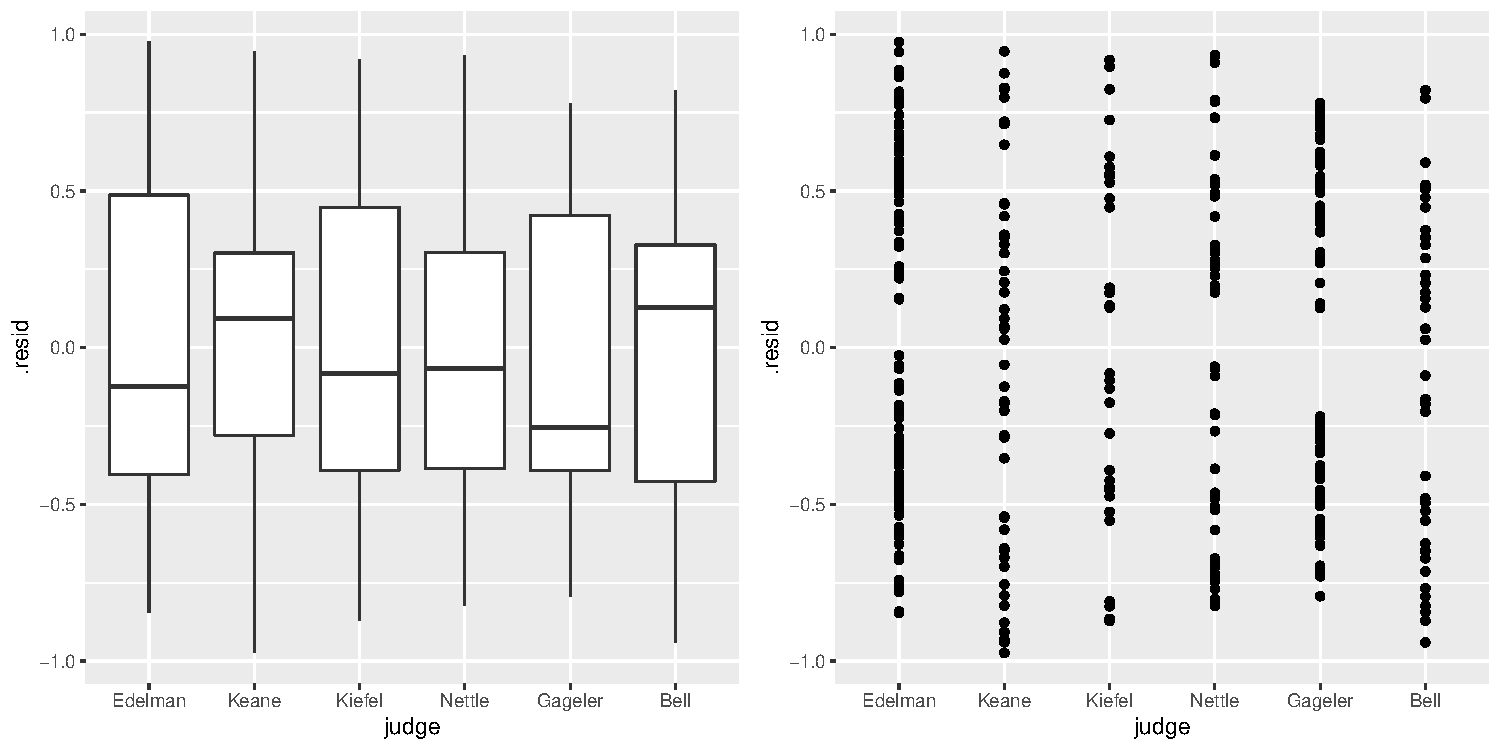
\includegraphics[width=1\linewidth]{figures/resid-judge-1} 

}

\caption{Residuals from Model 2 are graphed against judge. On the left panel, the mean of the residuals for each judge is close to zero and on the right panel, there is no clear pattern in the residuals can be observed. This indicates adequate fit.}\label{fig:resid-judge}
\end{figure}

\begin{figure}

{\centering 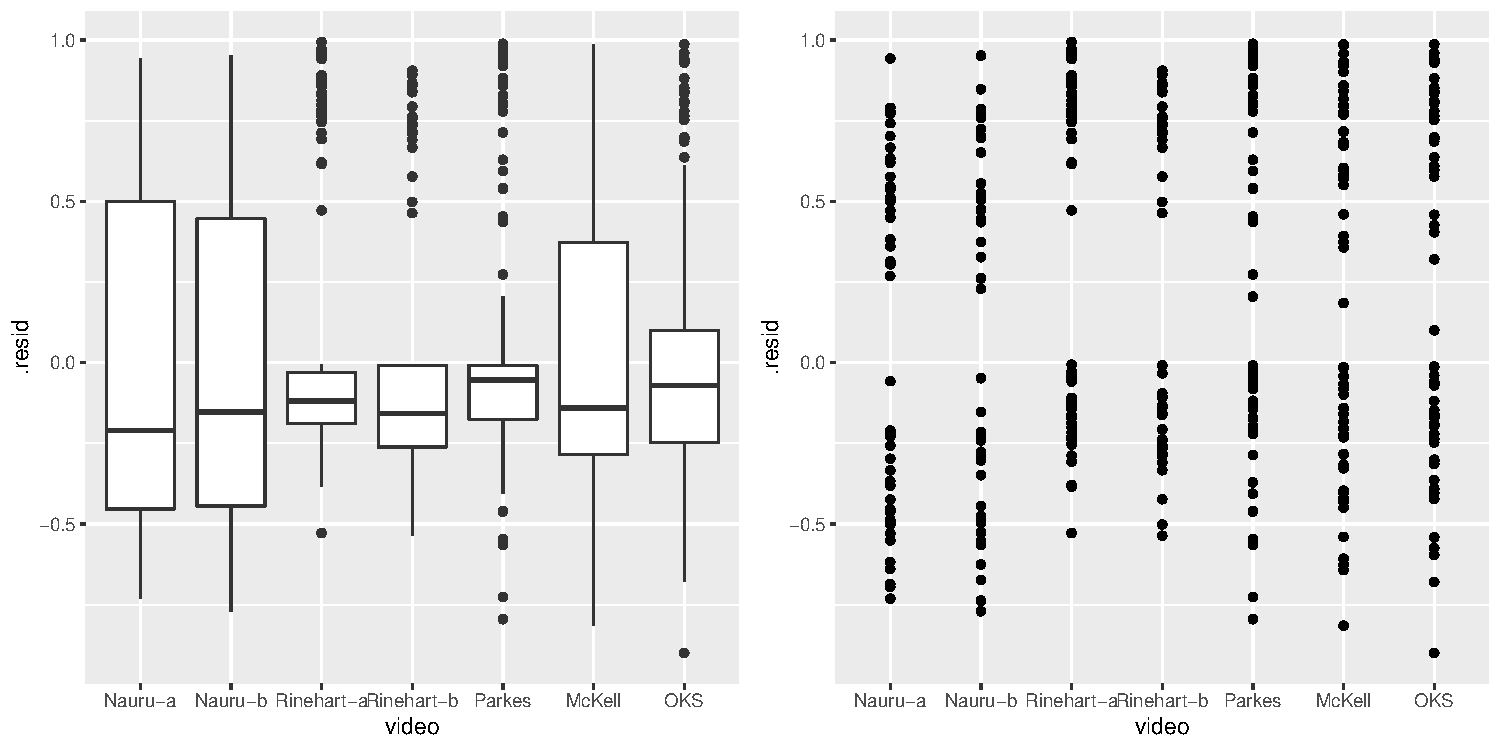
\includegraphics[width=1\linewidth]{figures/resid-video-1} 

}

\caption{Residuals from model 2 are graphed against video. There is no clear pattern in the residuals indicating adequate fit.}\label{fig:resid-video}
\end{figure}

\hypertarget{the-presence-of-facial-expression-of-the-justices-by-speaker}{%
\section{The presence of facial expression of the justices by speaker}\label{the-presence-of-facial-expression-of-the-justices-by-speaker}}

\begin{figure}

{\centering 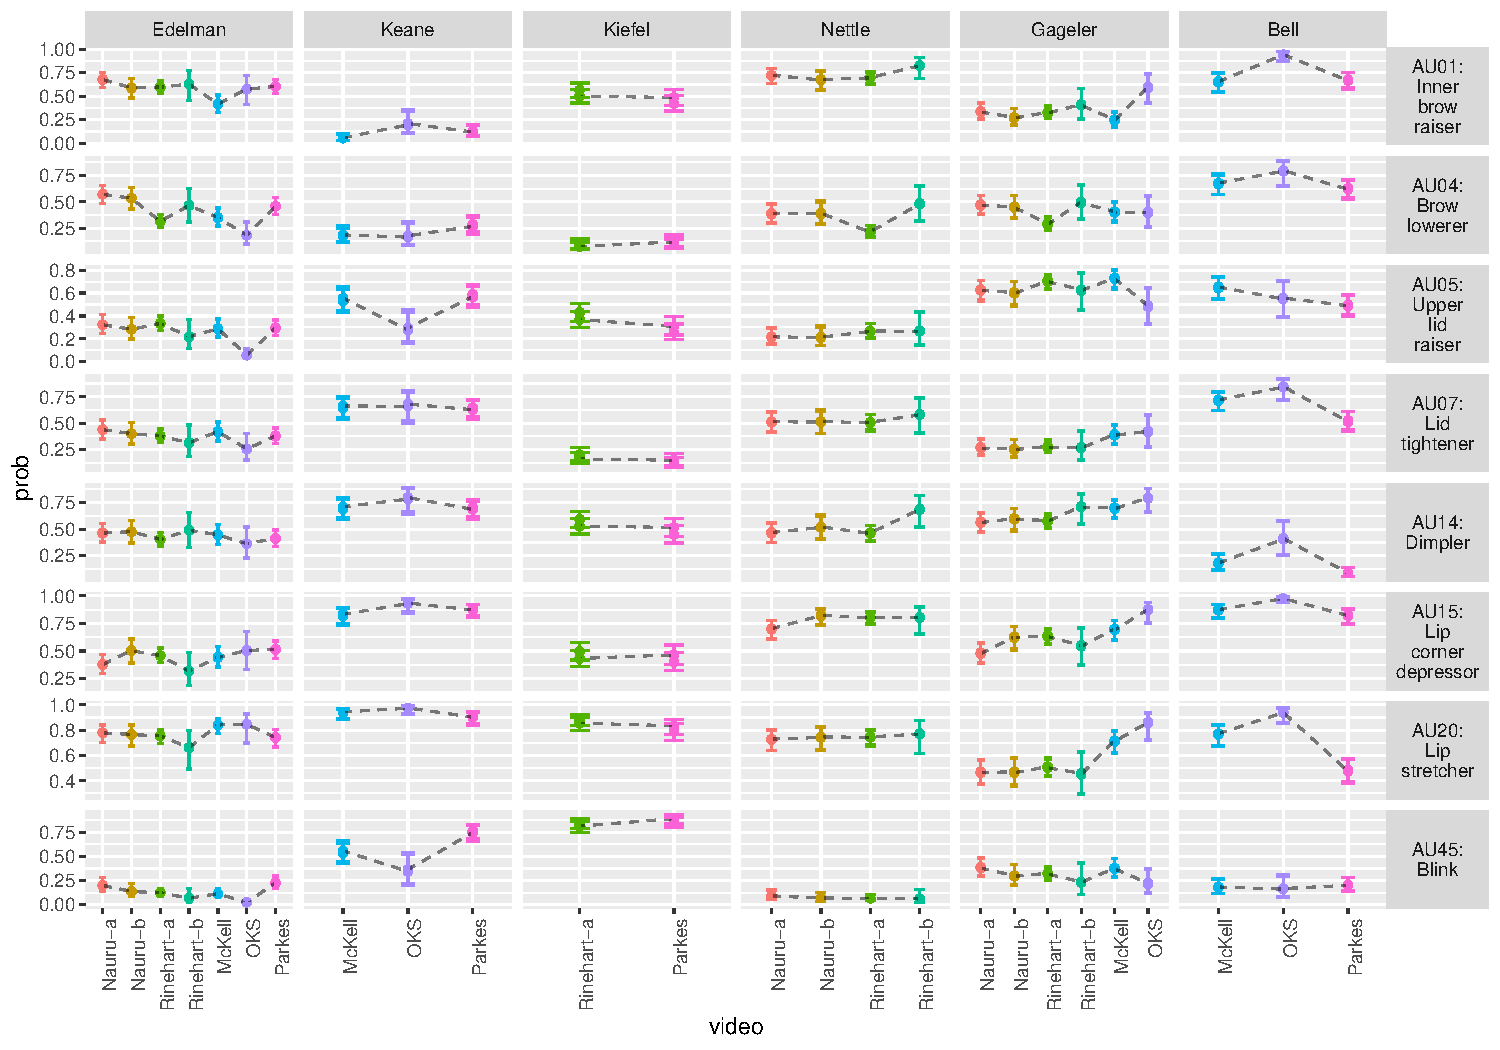
\includegraphics[width=1\linewidth]{figures/model3-plot-1} 

}

\caption{The 95\% confidence interval for estimated mearginal mean of presence after bonferroni adjustment. The x axis represents video and the y axis represents the estimated marginal mean of an action unit being observed. The facet shows the Justices in columns and action units in rows. The intervals for different speakers are overlaid with different colors. }\label{fig:model3-plot}
\end{figure}

\hypertarget{the-intensity-of-facial-expression-of-the-justices-by-speakers}{%
\section{The intensity of facial expression of the justices by speakers}\label{the-intensity-of-facial-expression-of-the-justices-by-speakers}}

\begin{figure}

{\centering 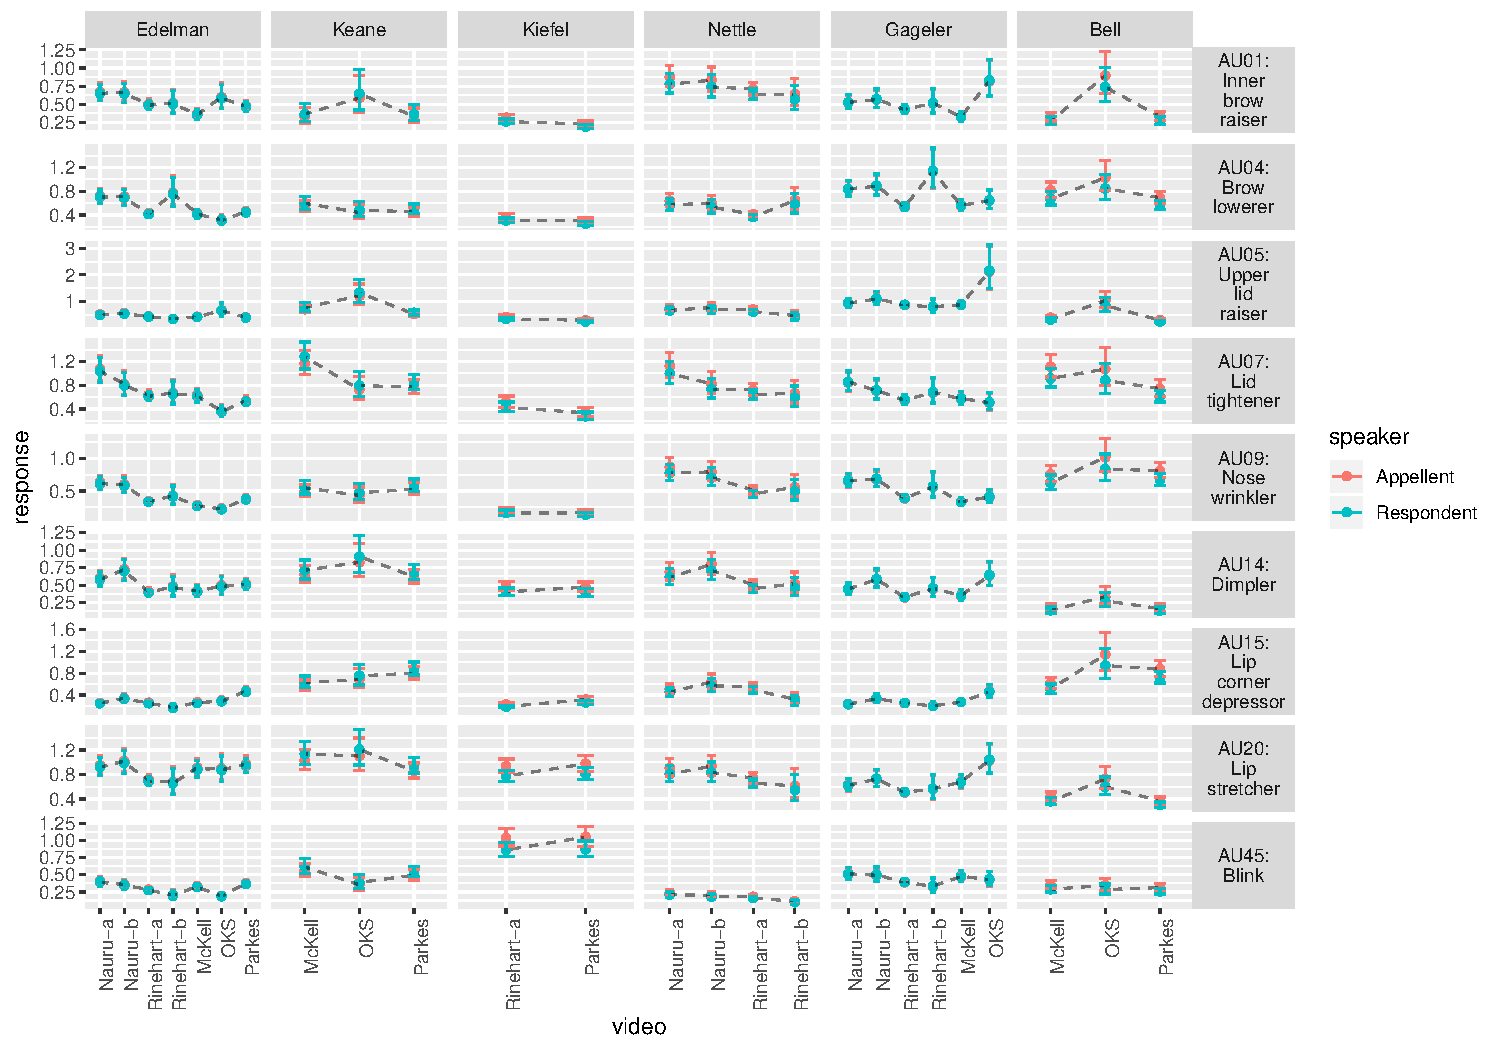
\includegraphics[width=1\linewidth]{figures/intensity-speaker-1} 

}

\caption{The 95\% confidence interval for estimated mearginal mean of intensity after bonferroni adjustment. The x axis represents video and the y axis represents the estimated marginal mean of the intensity. The facet shows the Justices in columns and action units in rows. The intervals for different speakers are overlaid with different colors.}\label{fig:intensity-speaker}
\end{figure}

\printbibliography[heading=bibintoc]


\end{document}
